\section{Pyramid}
\label{sec:Pyramid}

\begin{figure}[!ht]
\begin{center}
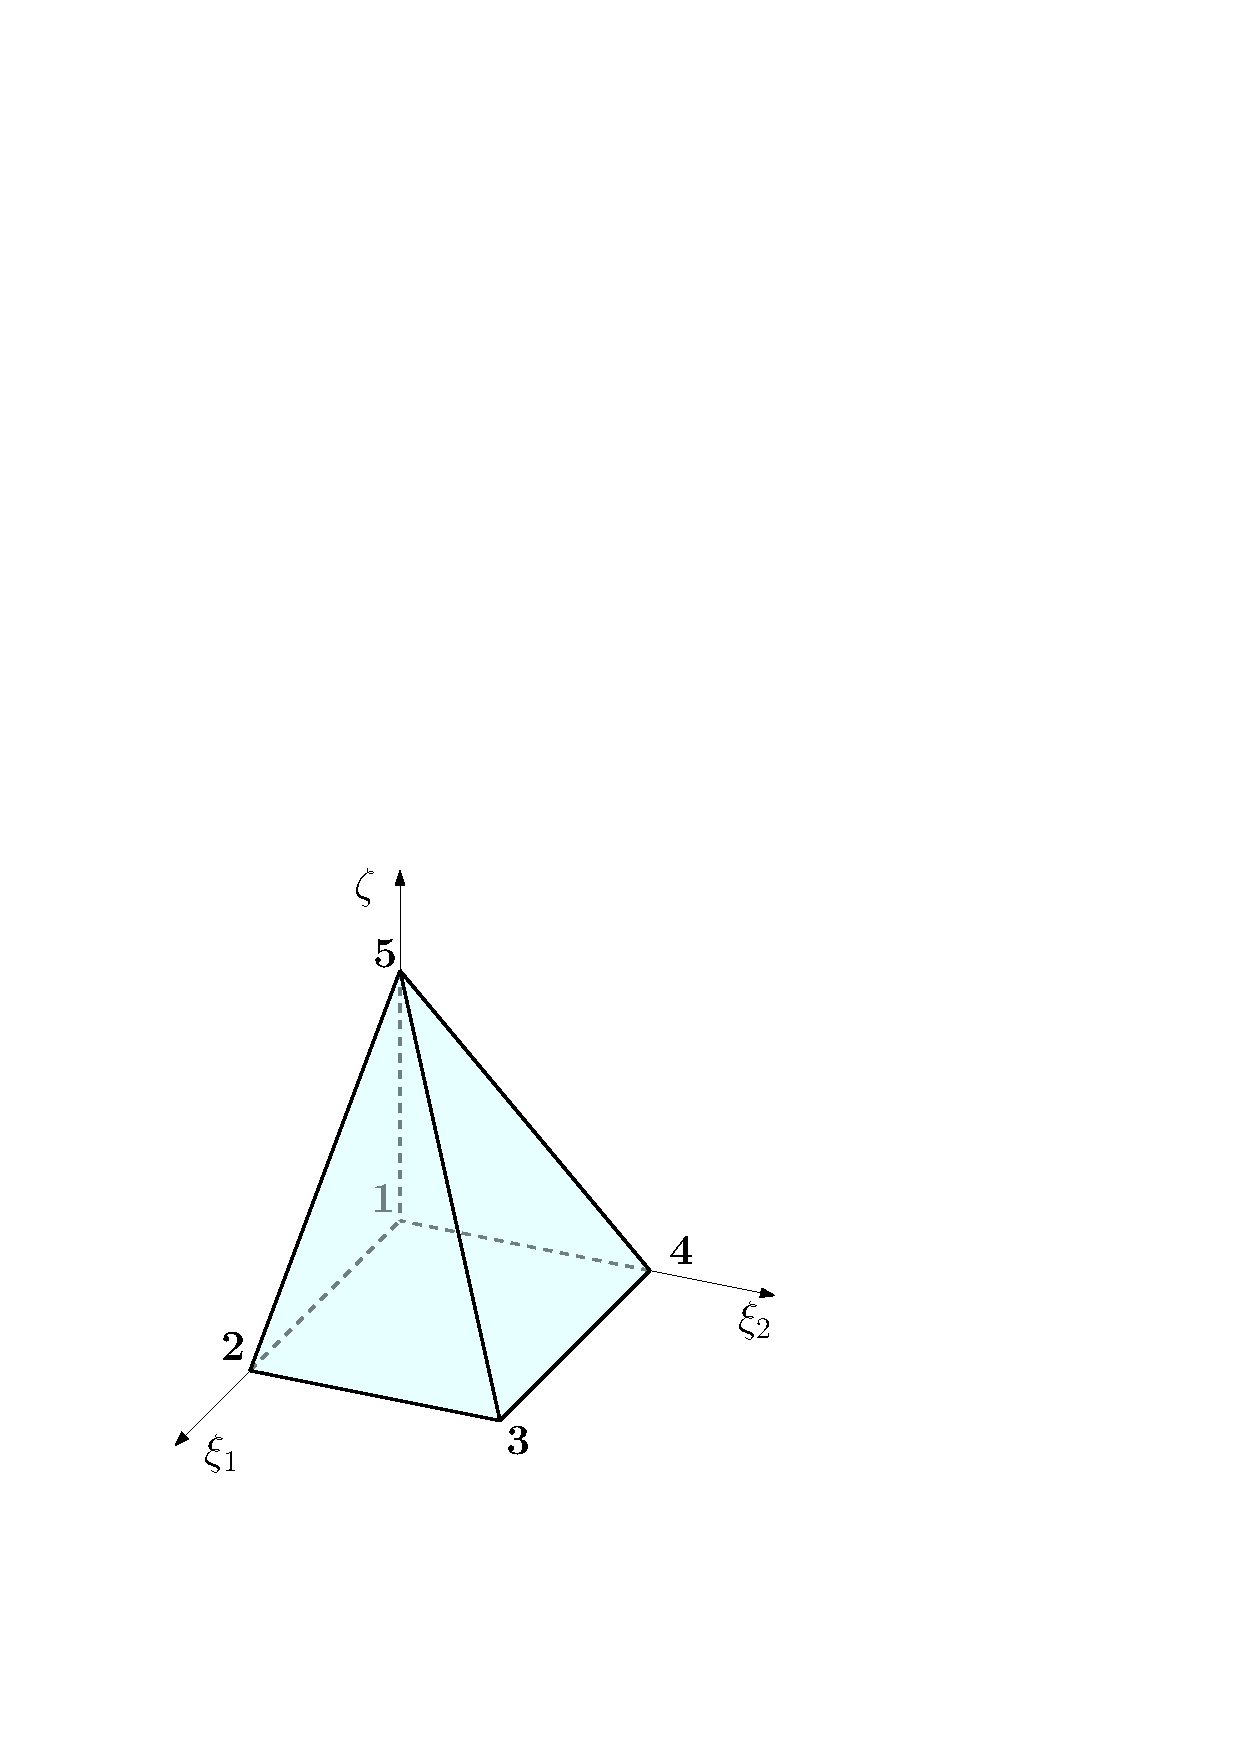
\includegraphics[scale=0.5]{./figures/MasterPyramid.pdf}
\caption{Master pyramid with numbered vertices.}
\label{fig:MasterPyramid}
\end{center}
\end{figure}

The master pyramid is shown in Figure \ref{fig:MasterPyramid} in the $(\xi,\zeta)=(\xi_1,\xi_2,\zeta)$ space.
More specifically, the definition is $\{(\xi_1,\xi_2,\zeta)\in\R^3:\xi_1>0,\xi_2>0,\zeta>0,\xi_1+\zeta<1,\xi_2+\zeta<1\}$.

Clearly, the pyramid is neither a simplex nor a Cartesian product, but it captures features of both quadrilaterals and triangles.
Indeed, it has both quadrilateral and triangle faces. 
Similarly, it has two types of edges. 
Those edges which are adjacent to both a quadrilateral face and a triangle face are called \textit{mixed edges}, while those edges only shared by triangle faces alone are called \textit{triangle edges}. 
These distinctions are fundamental, and the form of the shape functions will differ for the different types of edges and faces.

Due to the virtually unknown structure of the pyramid, at first it seems almost like an insurmountable task to be able to find representative functions that resemble affine coordinates for this 3D element. 
Surprisingly, there is in fact such a set (or rather set\textit{s}) of coordinates.
However, to reach that point, it is better to start by elementary means.
With this in mind, the idea is to separately analyze the affine coordinates of the quadrilateral face and the triangle faces.

In truth, nothing is getting in the way of explicitly computing the 2D triangle affine coordinates of each of the four triangle faces as described in \S\ref{sec:affinecoordinates}.
There turns out to be two independent sets of such coordinates which are
\begin{equation}
	\begin{gathered}
		\nu_0(\xi_1,\zeta)=1-\xi_1-\zeta\,,\qquad\nu_1(\xi_1,\zeta)=\xi_1\,,\qquad\nu_2(\zeta)=\zeta\,,\\
		\nu_0(\xi_2,\zeta)=1-\xi_2-\zeta\,,\qquad\nu_1(\xi_2,\zeta)=\xi_2\,,\qquad\nu_2(\zeta)=\zeta\,.
	\end{gathered}
	\label{eq:PyramidTriCoord}
\end{equation}
Indeed, the triplet $\vec{\nu}_{012}(\xi_1,\zeta)$ represents triangle faces 125 and 435, while the triplet $\vec{\nu}_{012}(\xi_2,\zeta)$ represents triangle faces 145 and 235.
Their gradient is
\begin{equation}
	\begin{gathered}
		\nabla\nu_0(\xi_1,\zeta)=\bigg(\begin{smallmatrix}-1\\[2pt]0\\[2pt]-1\end{smallmatrix}\bigg)\,,\qquad
			\nabla\nu_1(\xi_1,\zeta)=\bigg(\begin{smallmatrix}1\\[2pt]0\\[2pt]0\end{smallmatrix}\bigg)\,,\qquad
				\nabla\nu_2(\zeta)=\bigg(\begin{smallmatrix}0\\[2pt]0\\[2pt]1\end{smallmatrix}\bigg)\,,\\
		\nabla\nu_0(\xi_2,\zeta)=\bigg(\begin{smallmatrix}0\\[2pt]-1\\[2pt]-1\end{smallmatrix}\bigg)\,,\qquad
			\nabla\nu_1(\xi_2,\zeta)=\bigg(\begin{smallmatrix}0\\[2pt]1\\[2pt]0\end{smallmatrix}\bigg)\,,\qquad
				\nabla\nu_2(\zeta)=\bigg(\begin{smallmatrix}0\\[2pt]0\\[2pt]1\end{smallmatrix}\bigg)\,.
	\end{gathered}
	\label{eq:PyramidTriCoordGrad}
\end{equation}

Now, the quadrilateral face can undergo a similar treatment, resulting in the standard two sets of 1D affine coordinates,
\begin{equation*}
	\begin{gathered}
		\mu_0(\xi_1)=1-\xi_1\,,\quad\qquad\mu_1(\xi_1)=\xi_1\,,\\
		\mu_0(\xi_2)=1-\xi_2\,,\quad\qquad\mu_1(\xi_2)=\xi_2\,.
	\end{gathered}
\end{equation*}
However, these are convenient only when restricted to the 2D quadrilateral face, and not in 3D.
The reason is that they do \textit{not} act as blending functions to the \textit{faces}.
For example, $\mu_0(\xi_2)$ is unity at face 125, but it does \textit{not} vanish at the opposite face, which is face 435.
This inconvenience does not occur with the hexahedron or prism due to the Cartesian product structure of those elements.
Despite this setback, it is possible to fix this by considering \textit{scaled} coordinates which additionally depend on $\zeta$.
The sets of quadrilateral scaled 1D affine coordinates are
\begin{equation}
	\begin{gathered}
		\mu_0(\sxi)=1-\sxi\,,\quad\qquad\mu_1(\sxi)=\sxi\,,\\
		\mu_0(\sxii)=1-\sxii\,,\quad\qquad\mu_1(\sxii)=\sxii\,.
	\end{gathered}
	\label{eq:PyramidQuadCoord}
\end{equation}
These can be readily checked to act as \textit{face} blending functions between the opposite triangular faces, which is precisely what was desired.
Moreover, when restricted to the quadrilateral face, so $\zeta=0$, they coincide with the usual sets of affine coordinates for the 2D quadrilateral faces.
Their gradient is
\begin{equation}
	\begin{gathered}
		\nabla\mu_0(\sxi)=\frac{1}{(1-\zeta)^2}\bigg(\begin{smallmatrix}-(1-\zeta)\\[2pt]0\\[2pt]-\xi_1\end{smallmatrix}\bigg)\,,\quad\qquad
    	\nabla\mu_1(\sxi)=\frac{1}{(1-\zeta)^2}\bigg(\begin{smallmatrix}(1-\zeta)\\[2pt]0\\[2pt]\xi_1\end{smallmatrix}\bigg)\,,\\
		\nabla\mu_0(\sxii)=\frac{1}{(1-\zeta)^2}\bigg(\begin{smallmatrix}0\\[2pt]-(1-\zeta)\\[2pt]-\xi_2\end{smallmatrix}\bigg)\,,\quad\qquad
    	\nabla\mu_1(\sxii)=\frac{1}{(1-\zeta)^2}\bigg(\begin{smallmatrix}0\\[2pt](1-\zeta)\\[2pt]\xi_2\end{smallmatrix}\bigg)\,.
	\end{gathered}
	\label{eq:PyramidQuadCoordGrad}
\end{equation}

Lastly, the 1D affine coordinates associated to the nonquadrilateral (top) vertex and the perpendicularly projected point to the quadrilateral face are
\begin{equation}
		\mu_0(\zeta)=1-\zeta\,,\quad\qquad\mu_1(\zeta)=\zeta\,.
		\label{eq:PyramidZCoord}
\end{equation}
Their gradient is
\begin{equation}
		\nabla\mu_0(\zeta)=\bigg(\begin{smallmatrix}0\\[2pt]0\\[2pt]-1\end{smallmatrix}\bigg)\,,\quad\qquad
			\nabla\mu_1(\zeta)=\bigg(\begin{smallmatrix}0\\[2pt]0\\[2pt]1\end{smallmatrix}\bigg)\,.
		\label{eq:PyramidZCoordGrad}			
\end{equation}

With these tools in the arsenal, it is possible to find the desired 3D affine-like coordinates.
The first key observation is that each vertex in the quadrilateral face is associated to \textit{four} lower dimensional affine coordinates.
The associated coordinates are those which take the value $1$ at the given vertex.
For example, vertex $v_1=(0,0,0)$ is linked to the coordinates $\nu_0(\xi_1,\zeta)$, $\nu_0(\xi_2,\zeta)$, $\mu_0(\sxi)$ and $\mu_0(\sxii)$.
To find a global coordinate associated to any vertex, the idea is to combine these components such that they vanish at all disjoint edges and faces.
One possibility is to consider the product of all four coordinates.
However, this gives a high order function, which is somewhat inconsistent with what one would expect.
Hence, the global coordinate should look as ``simple'' as possible.
Fortunately, there is such a coordinate, which in fact has a dual interpretation with respect to its associated coordinates.
It is the product of a 1D scaled affine coordinate and the complementing 2D affine coordinate.
For vertex $v_0$, it would either be $\mu_0(\sxi)\nu_0(\xi_2,\zeta)$ or $\mu_0(\sxii)\nu_0(\xi_1,\zeta)$. 
These two interpretations coincide and define the pyramid affine-related coordinates.
For the nonquadrilateral vertex, $v_5=(0,0,1)$, there is an already existing affine-related coordinate which is merely $\nu_2(\zeta)=\mu_1(\zeta)$.
In summary, the pyramid affine-related coordinates are
\begin{equation}
	\begin{alignedat}{5}
		&\lambda_1(\xi,\zeta)&&=\mu_0(\sxi)\nu_0(\xi_2,\zeta)&&=\mu_0(\sxii)\nu_0(\xi_1,\zeta)
			&&=\textstyle{\frac{(1-\xi_1-\zeta)(1-\xi_2-\zeta)}{1-\zeta}}\,,\\
		&\lambda_2(\xi,\zeta)&&=\mu_1(\sxi)\nu_0(\xi_2,\zeta)&&=\mu_0(\sxii)\nu_1(\xi_1,\zeta)
			&&=\textstyle{\frac{\xi_1(1-\xi_2-\zeta)}{1-\zeta}}\,,\\
		&\lambda_3(\xi,\zeta)&&=\mu_1(\sxi)\nu_1(\xi_2,\zeta)&&=\mu_1(\sxii)\nu_1(\xi_1,\zeta)
			&&=\textstyle{\frac{\xi_1\xi_2}{1-\zeta}}\,,\\
		&\lambda_4(\xi,\zeta)&&=\mu_0(\sxi)\nu_1(\xi_2,\zeta)&&=\mu_1(\sxii)\nu_0(\xi_1,\zeta)
			&&=\textstyle{\frac{(1-\xi_1-\zeta)\xi_2}{1-\zeta}}\,,\\
		&\lambda_5(\zeta)&&=\nu_2(\zeta)&&=\mu_1(\zeta)&&=\zeta\,.
	\end{alignedat}
	\label{eq:PyramidAffineCoord}
\end{equation}
Their gradient is
\begin{equation}
	\begin{gathered}
    \nabla\lambda_1(\xi,\zeta)=\begin{pmatrix}\frac{-(1-\xi_2-\zeta)}{1-\zeta}\\\frac{-(1 -\xi_1-\zeta)}{1-\zeta}\\
        \frac{\xi_1\xi_2}{(1-\zeta)^2}-1\end{pmatrix}\,,\quad
    \nabla\lambda_2(\xi,\zeta)=\begin{pmatrix}\frac{(1-\xi_2-\zeta)}{1-\zeta}\\\frac{-\xi_1}{1-\zeta}\\
        \frac{-\xi_1\xi_2}{(1-\zeta)^2}\end{pmatrix}\,,\quad
    \nabla\lambda_3(\xi,\zeta)=\begin{pmatrix}\frac{\xi_2}{1-\zeta}\\\frac{\xi_1}{1-\zeta}\\
        \frac{\xi_1\xi_2}{(1-\zeta)^2}\end{pmatrix}\,,\\
    \nabla\lambda_4(\xi,\zeta)=\begin{pmatrix}\frac{-\xi_2}{1-\zeta}\\\frac{(1-\xi_1-\zeta)}{1-\zeta}\\
        \frac{-\xi_1\xi_2}{(1-\zeta)^2}\end{pmatrix}\,,\quad
    \nabla\lambda_5(\zeta)=\begin{pmatrix}0\\0\\1\end{pmatrix}\,.
	\end{gathered}
	\label{eq:PyramidAffineCoordGrad}
\end{equation}

Apart from being products of lower dimensional affine coordinates, the pyramid affine-related coordinates truly do behave in many ways like 3D affine coordinates.
Firstly, notice that by construction the traces over adjacent faces and edges are the corresponding vertex functions of those lower dimensional topological entities.
For example, the trace of $\lambda_1$ over faces 125 and 145 is a 2D triangle affine coordinate associated to that vertex, while that of face 1234 is a bilinear quadrilateral vertex function.
Secondly, note that every $(\xi,\zeta)$ in the pyramid can be expressed as a convex combination of the vertices with the affine coordinates being the weights,
\begin{equation}
	\bigg(\begin{smallmatrix}\xi_1\\[2pt]\xi_2\\[2pt]\zeta\end{smallmatrix}\bigg)=\sum_{a=1}^5 \lambda_a(\xi,\zeta)v_a\,,
		\qquad\quad\text{ with }\quad\sum_{a=1}^5 \lambda_a(\xi,\zeta)=1\,\;\text{ and }\; 0\leq\lambda_a(\xi,\zeta)\leq1\,,
\end{equation}
and where $v_a$ are the coordinates of vertex $a$. 
The main difference with the legitimate simplex affine coordinates radicates in the fact the the pyramid affine-related coordinates are not \textit{defined} by the properties above (see \S\ref{sec:affinecoordinates}).
Indeed, even though they have polynomial traces at the boundary, they involve rational polynomials in the interior, and this is an inherently new property.
Nevertheless, for many practical purposes, they can be thought of as affine coordinates, and from now on will be referred to as \textit{the} pyramid affine coordinates.

An important remark is that all the results associated to the definitions of the ancillary functions were proved in a very general setting that encompasses the pyramid affine coordinates and the fact they can be rational. 
In particular, the proofs of Lemmas \ref{lem:curlformula} and \ref{lem:divformula} hold.

Note that all the affine coordinates illustrated can be computed for pyramids with a parallelogram base.
In fact, it is very easy to make these calculations for pyramids with an arbitrarily placed top vertex and whose rectangular base is normal to the vertical $\zeta$ direction and aligned with the $\xi$ coordinates.
This assertion includes any of the typical master pyramids found in the literature.
With the affine coordinates computed, it is just a matter of substituting them (and their gradient) into the expressions for the shape functions to be presented throughout this section, so that in fact these expressions are independent of the choice of the master pyramid.
Hopefully, this motivates other researchers to communicate their results in terms of affine coordinates as well.

Finally, by construction, there are natural relationships between the topological entities and the different types of affine coordinates defined.
The related affine coordinates are those which take the value $1$ at the prescribed topological entity.
The top vertex, $v_5$, is linked to $\nu_2(\zeta)=\mu_1(\zeta)=\lambda_5(\zeta)$.
The quadrilateral vertices are each associated to \textit{two} 1D scaled affine coordinates, \textit{two} 2D triangle affine coordinates and \textit{one} 3D pyramid affine coordinate.
Meanwhile, triangle edges are linked to \textit{two} 1D scaled affine coordinates, while mixed edges are associated to \textit{one} 1D scaled affine coordinate and the vertical 1D affine coordinate $\mu_0(\zeta)$.
Lastly, triangle faces are linked to \textit{one} 1D scaled affine coordinate, while the quadrilateral face is linked to the vertical 1D affine coordinate $\mu_0(\zeta)$.
As usual, these associated affine coordinates can act as natural blending functions.

\subsubsection*{Exact Sequence}

It should be clear by now that the pyramid has a fundamentally different structure than the previous elements, and one would expect this to have an impact on the discrete spaces that attempt to approximate the energy spaces in \eqref{eq:3D_exact_sequence}.

Firstly, note that an absolute requirement is that the trace of the spaces over the faces span the lower dimensional discrete polynomial spaces for the triangle and quadrilateral respectively.
This is what ensures that the shape functions are compatible over adjacent elements.
However, any attempt at finding a three dimensional polynomial space satisying those properties is futile, since one can find counterexamples mathematically showing that this task is impossible.

Hence, the use of \textit{rational} polynomial spaces is the next natural step.
This issue already arised, at least intuitively, while analyzing the desired properties of affine coordinates, because the use of \textit{scaled} coordinates was required.
Nevertheless, dealing with rational polynomial spaces is difficult, and finding finite dimensional higher order spaces satisfying all the desired trace, exact sequence and approximability properties is a far from trivial task.
In fact, only until recently did such constructions started to appear in the literature.
In the context of this work, perhaps the best suited set of such spaces is that proposed by \citet{Nigam_Phillips_11}, which is consistent with the ``natural'' first order spaces analyzed first by \citet{Hiptmair99}.

Respecting the notation of \citet{Nigam_Phillips_11}, the discrete rational polynomial spaces approximating \eqref{eq:3D_exact_sequence} are,
\begin{equation}
	\mathcal{U}^{(0),p} \xrightarrow{\,\,\nabla\,\,} \mathcal{U}^{(1),p} \xrightarrow{\nabla\times} 
	\mathcal{U}^{(2),p} \xrightarrow{\nabla\cdot} \mathcal{U}^{(3),p} \,,
	\label{eq:pyramidsequence}
\end{equation}
where the $m$ in $\mathcal{U}^{(m),p}$ corresponds to the order of the differential form in 3D, so that the elements in $\mathcal{U}^{(0),p}$ are $0$-forms, and so on.
The precise definitions of these spaces are somewhat technical and will be postponed to Appendix \ref{app:pyrappendix}.
In fact, the proofs that the shape funtions lie in the desired space are also technical and inconveniently load the readibility of the document, so they are presented in Appendix \ref{app:pyrappendix} as well. 
This by no means implies that the spaces are not important and do not play a role in the construction.
In fact, quite the opposite.
The spaces are so well suited to the pyramid, that most of the time they impose little restrictions on the intuitive constructions presented here.
Hence, in many ways, despite looking complicated, they are ``natural''.

Finally, it is worth emphasizing that the goal in this section (and in general in this work) is to motivate the construction of the shape functions through geometrical arguments (via the affine coordinates defined before) combined with the carefully chosen ancillary operators defined throughout the document.
This approach leads to shape functions satisfying the desired trace properties and which either are in the desired space or can be naturally tweaked to lie in the space.
The notable exception is that of the $H(\mathrm{div})$ triangle faces, in which the space truly plays a nontrivial role and forces to consider a more intricate yet consistent construction.

%Having said this, there are exceptions.
%Notably, in the case of $H(\mathrm{div})$, the space truly plays a nontrivial role and forces to consider a more intricate construction for some shape functions.
%These exceptions will be pointed out.

%Hence, the focus will be on the geometric intuition and on how the logic of projecting, evaluating and blending applies to the shape functions in this element.
%The desired trace properties


%This approach leads to shape functions which are in the desired space or which can be intuitively modified to lie in the space.
%Hence, this speaks very well on the suitability and importance of these spaces for the pyramid, which in many ways can be considered `natural'.
%Having said this, there are exceptions.
%Notably, in the case of $H(\mathrm{div})$, the space truly plays a nontrivial role and forces to consider a more intricate construction for some shape functions.
%These exceptions will be pointed out.
%
%This by no means implies that 
%
%
%will all be given in Appendix \ref{app:pyrappendix}.
%
%The justification for this is that the construction of shape functions is fully motivated by geometrical arguments (via the affine coordinates defined before) combined with the carefully chosen ancillary operators defined throughout the document.
% 
%Hence, in many ways the space plays a `natural' role and imposes little restrictions on the construction.
%This speaks very well on the suitability of these spaces for the pyramid.
%However, the proofs that the shape functions are in the space are technical and inconveniently load the readibility of the document, which has the goal of motivating the shape functions through
%, that the aspect of conformability almost becomes superfluous.  
%This , but it is inconvenient to load the readibility of these proofs on of the document, they are given in Appendix \ref{app:pyrappendix}.
%Having said this, there are key exceptions in the case of $H(\mathrm{div})$, where the space truly plays a nontrivial role and forces to consider a more intricate construction.
%These exceptions will be pointed out.

\subsection{\texorpdfstring{$H^1$}{H1} Shape Functions}

The dimension of the space $\mathcal{U}^{(0),p}$ is $p^3+3p+1$.
The number of linearly independent shape functions will coincide with that dimension.

\subsubsection {\texorpdfstring{$H^1$}{H1} Vertices}

The vertex shape functions will be precisely the associated 3D pyramid affine coordinates.
Indeed, take for example vertex $v_1$, so that the vertex function is
\begin{equation*}
	\phi^\mathrm{v}(\xieta)=\lambda_1(\xieta)\,.
\end{equation*}
The trace properties are satisfied by construction and are shown explicitly next,
\begin{equation*}
	\begin{alignedat}{5}
    &\phi^\mathrm{v}(\xieta)|_{\xi_2=0}&&=\lambda_1(\xieta)|_{\mu_0(\frac{\xi_1}{1-\zeta})=1}
    	&&=\mu_0(\sxi)\nu_0(\xi_2,\zeta)|_{\mu_0(\frac{\xi_1}{1-\zeta})=1}&&=\nu_0(\xi_2,\zeta)\,,\\
    &\phi^\mathrm{v}(\xieta)|_{\xi_1=1-\zeta}&&=\lambda_1(\xieta)|_{\mu_0(\frac{\xi_2}{1-\zeta})=0}
    	&&=\mu_0(\sxii)\nu_0(\xi_1,\zeta)|_{\mu_0(\frac{\xi_2}{1-\zeta})=0}&&=0\,,\\
  	&\phi^\mathrm{v}(\xieta)|_{\xi_2=1-\zeta}&&=\lambda_1(\xieta)|_{\mu_0(\frac{\xi_1}{1-\zeta})=0}
    	&&=\mu_0(\sxi)\nu_0(\xi_2,\zeta)|_{\mu_0(\frac{\xi_1}{1-\zeta})=0}&&=0\,,\\
    &\phi^\mathrm{v}(\xieta)|_{\xi_2=0}&&=\lambda_1(\xieta)|_{\mu_0(\frac{\xi_2}{1-\zeta})=1}
    	&&=\mu_0(\sxii)\nu_0(\xi_1,\zeta)|_{\mu_0(\frac{\xi_2}{1-\zeta})=1}&&=\nu_0(\xi_1,\zeta)\,,\\
    &\phi^\mathrm{v}(\xieta)|_{\zeta=0}&&=\lambda_1(\xieta)|_{\zeta=0}
    	&&=\mu_0(\xi_1)\mu(\xi_2)\,.&&\\
	\end{alignedat}
\end{equation*}
The function is also in the lowest order space $\mathcal{U}^{(0),1}$.
Similar arguments apply to all other quadrilateral vertices and the top vertex as well.

More generally, the vertex functions and their gradient are,
\begin{equation}
    \phi^\mathrm{v}(\xieta)=\lambda_a(\xieta)\,,\qquad\quad\nabla\phi^\mathrm{v}(\xieta)=\nabla\lambda_a(\xieta)\,,
    \label{eq:PyrH1Vertex}
\end{equation}
for $a=1,2,3,4,5$.
There are a total of $5$ vertex functions (one for each vertex).

\subsubsection{\texorpdfstring{$H^1$}{H1} Edges}

\paragraph{\texorpdfstring{$H^1$}{H1} Mixed Edges.} 
Take for example mixed edge 12.
The first naive approach is to use the 3D pyramid affine coordinates directly on $\phi_i^\E$, which gives
\begin{equation*}
	\phi_i^\mathrm{e}(\xieta)=\phi_i^\E(\vec{\lambda}_{12}(\xieta))
		=\phi_i^\E\Big(\mu_0(\sxii)\nu_0(\xi_1,\zeta),\mu_0(\sxii)\nu_1(\xi_1,\zeta)\Big)
			=\mu_0(\sxii)^i\phi_i^\E(\vec{\nu}_{01}(\xi_1,\zeta))\,,
\end{equation*}
for $i=2,\ldots,p$.
This attempt almost works because it is in the correct space, satisfies the vanishing conditions, and even has the right form at the edge itself.
Indeed, at triangle faces 235 and 145, $\nu_0(\xi_1,\zeta)=0$ and $\nu_1(\xi_1,\zeta)=0$ respectively, while $\mu_0(\sxii)=0$ at face 435.
However, the nonzero trace over the adjacent quadrilateral face is not of the correct form, since it blends nonlinearly with the factor $\mu_0(\xi_2)^i$ instead of linearly like $\mu_0(\xi_2)$.
Therefore the function violates dimensional hierarchy and does not work for our purposes.
Nevertheless this analysis ellucidates how to fix the issue.
The idea is to have the factor $\mu_0(\sxii)$ separated as a blending factor, so that the effects of $\mu_0(\sxii)$ are essentially separated from those of $\vec{\nu}_{01}(\xi_1,\zeta)$ in $\vec{\lambda}_{12}(\xieta)$.
%This can always be done because of the decomposition of the 3D pyramid affine coordinate into lower dimensional affine coordinates.
Hence, the shape functions for this edge are
\begin{equation*}
	\phi_i^\mathrm{e}(\xieta)=\mu_0(\sxii)\phi_i^\E(\vec{\nu}_{01}(\xi_1,\zeta))=
		\underbrace{\mu_0(\sxii)(\nu_0(\xi_1,\zeta)+\nu_1(\xi_1,\zeta))^i}_{\text{blend}}
    	\underbrace{\phi_i^\E\Big(\underbrace{\textstyle{\frac{1}{\nu_0(\xi_1,\zeta)+\nu_1(\xi_1,\zeta)}}
    		\vec{\nu}_{01}(\xi_1,\zeta)}_{\text{project}}\Big)}_{\text{evaluate}}\,,
\end{equation*}
for $i=2,\ldots,p$.
As with the previous candidate all vanishing properties are satisfied, but this time the nonzero trace properties are also easily seen to hold.
The projection being implied is
\begin{equation*}
	(\xi_1,\xi_2,\zeta)\;\longmapsto\;\begin{matrix}(\xi_1,0,\zeta)\\(\sxi,\sxii,0)\end{matrix}
		\;\longmapsto\;(\sxi,0,0)\,.
\end{equation*}
It is a two step projection, where the first step is to project to an adjacent face and the second is to project along that face to the given edge via the standard 2D edge projections (see Figures \ref{fig:QuadProjection} and \ref{fig:TriangleProjection}).
If the face projection is chosen as the triangle, then the projection at play is called the \textit{horizontal} triangle face projection and consists of finding the intersection $P'=(\xi_1,0,\zeta)$ of the face with the projecting line parallel to the $\xi_2$ direction and passing through the original point $P=(\xi_1,\xi_2,\zeta)$. 
This is shown in Figure \ref{fig:PyramidProjectionHorizontalTriangle}.
If the face projection is chosen as the quadrilateral, then the projection is simply the intersection $P'=(\sxi,\sxii,0)$ of the face with the projecting line passing through the top vertex and the original point $P=(\xi_1,\xi_2,\zeta)$. 
This is shown in Figure \ref{fig:PyramidProjectionQuad}.

\begin{figure}[!ht]
\begin{center}
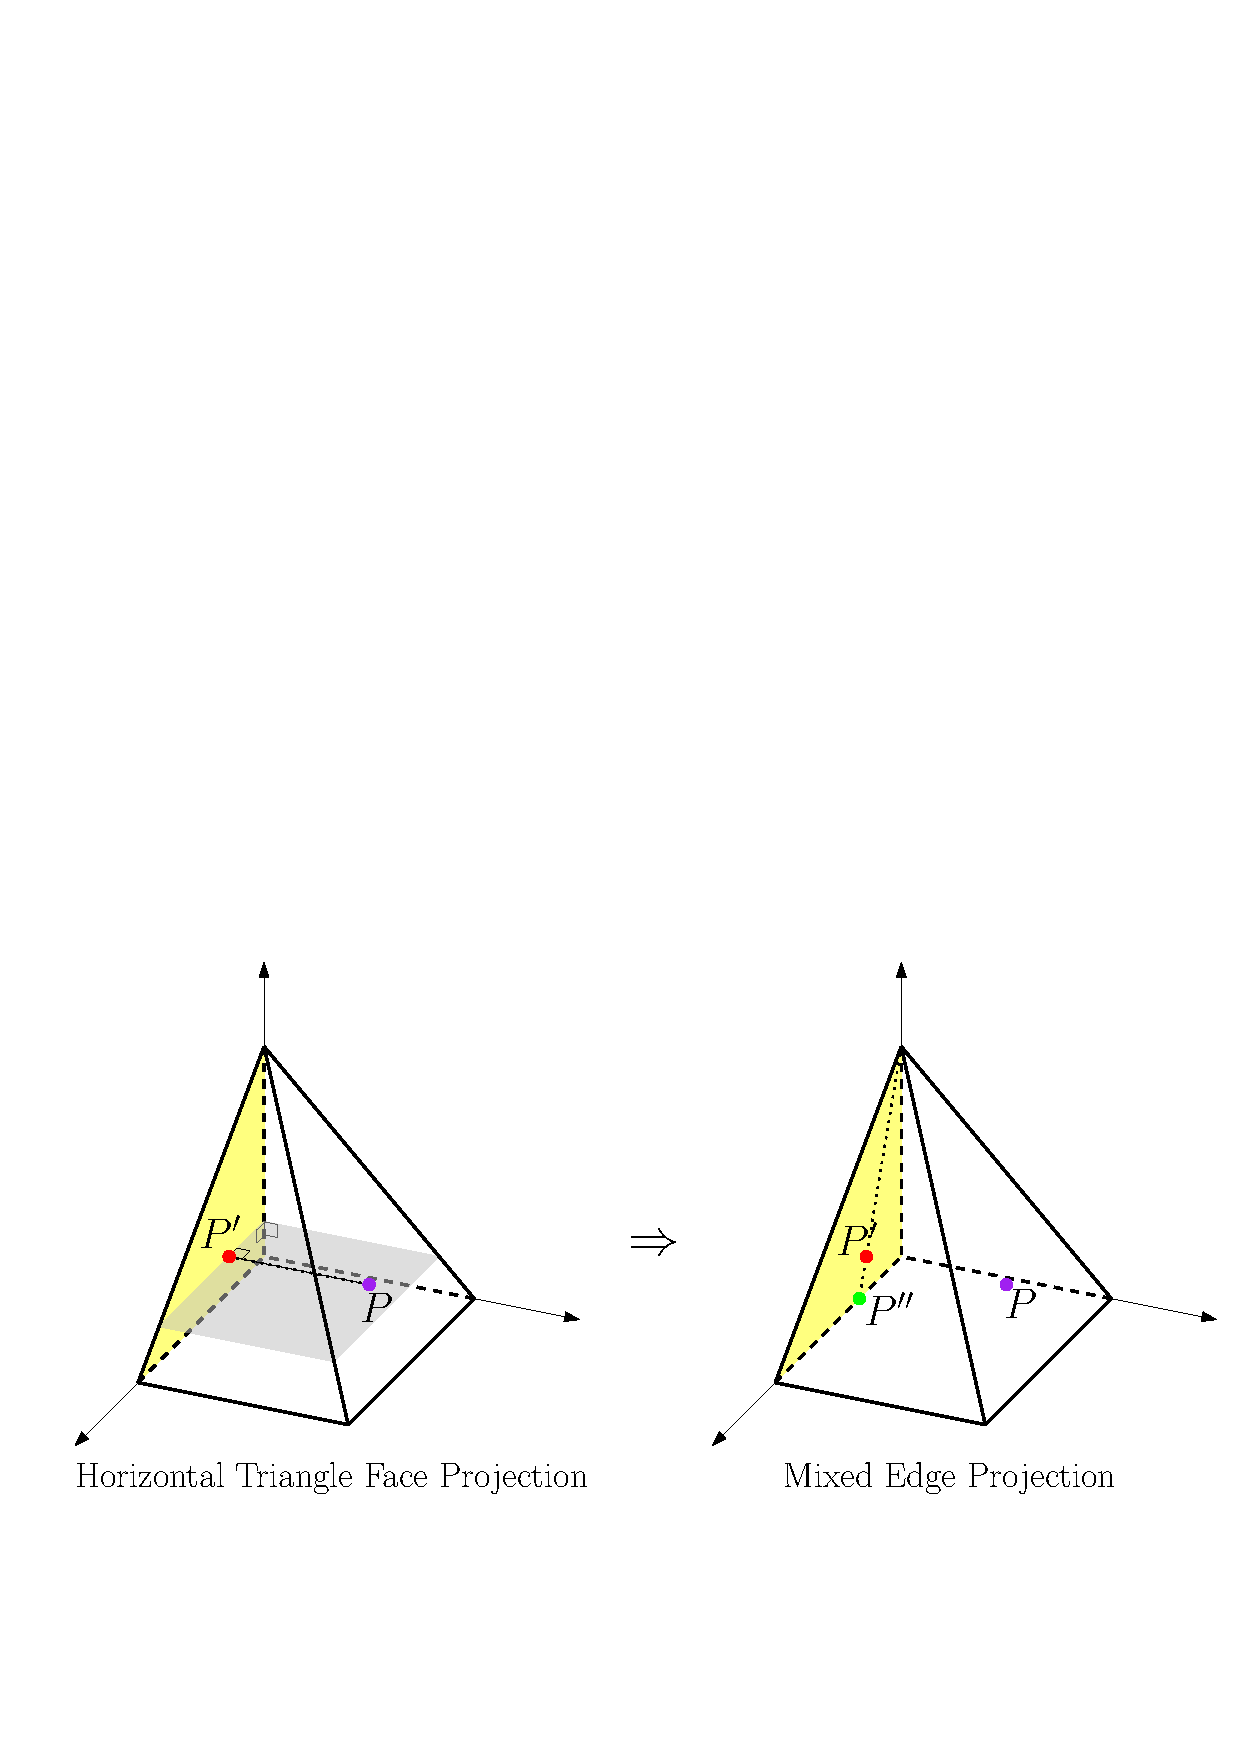
\includegraphics[scale=0.6]{./figures/PyramidProjectionHorizontalTriangle.pdf}
\caption{Horizontal triangle face projection from $P$ to $P'$ followed by a mixed edge projection from $P'$ to $P''$.}
\label{fig:PyramidProjectionHorizontalTriangle}
\end{center}
\end{figure}

In general, the shape functions and their gradient are
\begin{equation}
	\begin{aligned}
		\phi_i^\mathrm{e}(\xieta)&=\mu_c(\sxib)\phi_i^\E(\vec{\nu}_{01}(\xi_a,\zeta))\,,\\
    	\nabla\phi_i^\mathrm{e}(\xieta)&=\mu_c(\sxib)\nabla\phi_i^\E(\vec{\nu}_{01}(\xi_a,\zeta))
        +\phi_i^\E(\vec{\nu}_{01}(\xi_a,\zeta))\nabla\mu_c(\sxib)\,,	
	\end{aligned}
	\label{eq:PyrH1MixedEdge}
\end{equation}
where $i=2,\ldots,p$, $(a,b)=(1,2),(2,1)$ and $c=0,1$.
There are $p-1$ edge function for each edge, for a total of $4(p-1)$ mixed edge functions.

\paragraph{\texorpdfstring{$H^1$}{H1} Triangle Edges.}
For instance, take triangle edge 15.
Again, the naive approach is to use the 3D pyramid affine coordinates on $\phi_i^\E$, leading to the shape functions,
\begin{equation*}
	\phi^\mathrm{e}(\xieta)=\phi_i^\E(\vec{\lambda}_{15}(\xieta))=
		\underbrace{(\lambda_1(\xieta)+\lambda_5(\zeta))^i}_{\text{blend}}
    	\underbrace{\phi_i^\E\Big(\underbrace{\textstyle{\frac{1}{\lambda_1(\xieta)+\lambda_5(\zeta)}}
    		\vec{\lambda}_{15}(\xieta)}_{\text{project}}\Big)}_{\text{evaluate}}\,,
\end{equation*}
for $i=2,\ldots,p$.
In this case it works perfectly well, with the trace properties being satisfied.
Indeed, $\lambda_1(\xieta)=0$ over faces 235 and 435, while $\lambda_5(\xieta)=0$ over the quadrilateral face.
Moreover the restriction of $\vec{\lambda}_{15}(\xieta)$ over the faces 125 and 145 gives $\vec{\nu}_{02}(\xi_1,\zeta)$ and $\vec{\nu}_{02}(\xi_2,\zeta)$ respectively, so the nonzero traces are the appropriate triangle traces.
The projection being implied here is highly nontrivial. 
It is a two step projection given by
\begin{equation*}
	(\xi_1,\xi_2,\zeta)\;\longmapsto\;\Big(\textstyle{\frac{\xi_1(1-\xi_2-\zeta)}{(1-\xi_2)(1-\zeta)}},
		0,\textstyle{\frac{\zeta}{1-\xi_2}}\Big)\;\longmapsto\;
			\Big(0,0,\textstyle{\frac{\zeta(1-\zeta)}{(1-\xi_1-\zeta)(1-\xi_2-\zeta)+\zeta(1-\zeta)}}\Big)\,.
\end{equation*}
The first step is called an \textit{oblique} triangle face projection and consists of running a plane through the original point $P=(\xi_1,\xi_2,\zeta)$ and the opposite bottom edge to the face (edge 43), followed by finding the intersection of this plane with the planes passing through the other two adjacent triangular faces (faces 235 and 415 with equations $\xi_1=1-\zeta$ and $\xi_1=0$ respectively).
Call this intersection $C=(0,-(\frac{1-\xi_2-\zeta}{\zeta}),1)$.
Finally, the intersection of face 125 with the projecting line from the original point $P$ to the intersection $C$ is found and labeled as $P'=(\frac{\xi_1(1-\xi_2-\zeta)}{(1-\xi_2)(1-\zeta)},0,\frac{\zeta}{1-\xi_2})$.
This projection is illustrated in Figure \ref{fig:PyramidProjectionObliqueTriangle}.
The final step is simply to project as usual along the 2D triangle face to the point $P''=(0,0,\frac{\zeta(1-\zeta)}{(1-\xi_1-\zeta)(1-\xi_2-\zeta)+\zeta(1-\zeta)})$.

\begin{figure}[!ht]
\begin{center}
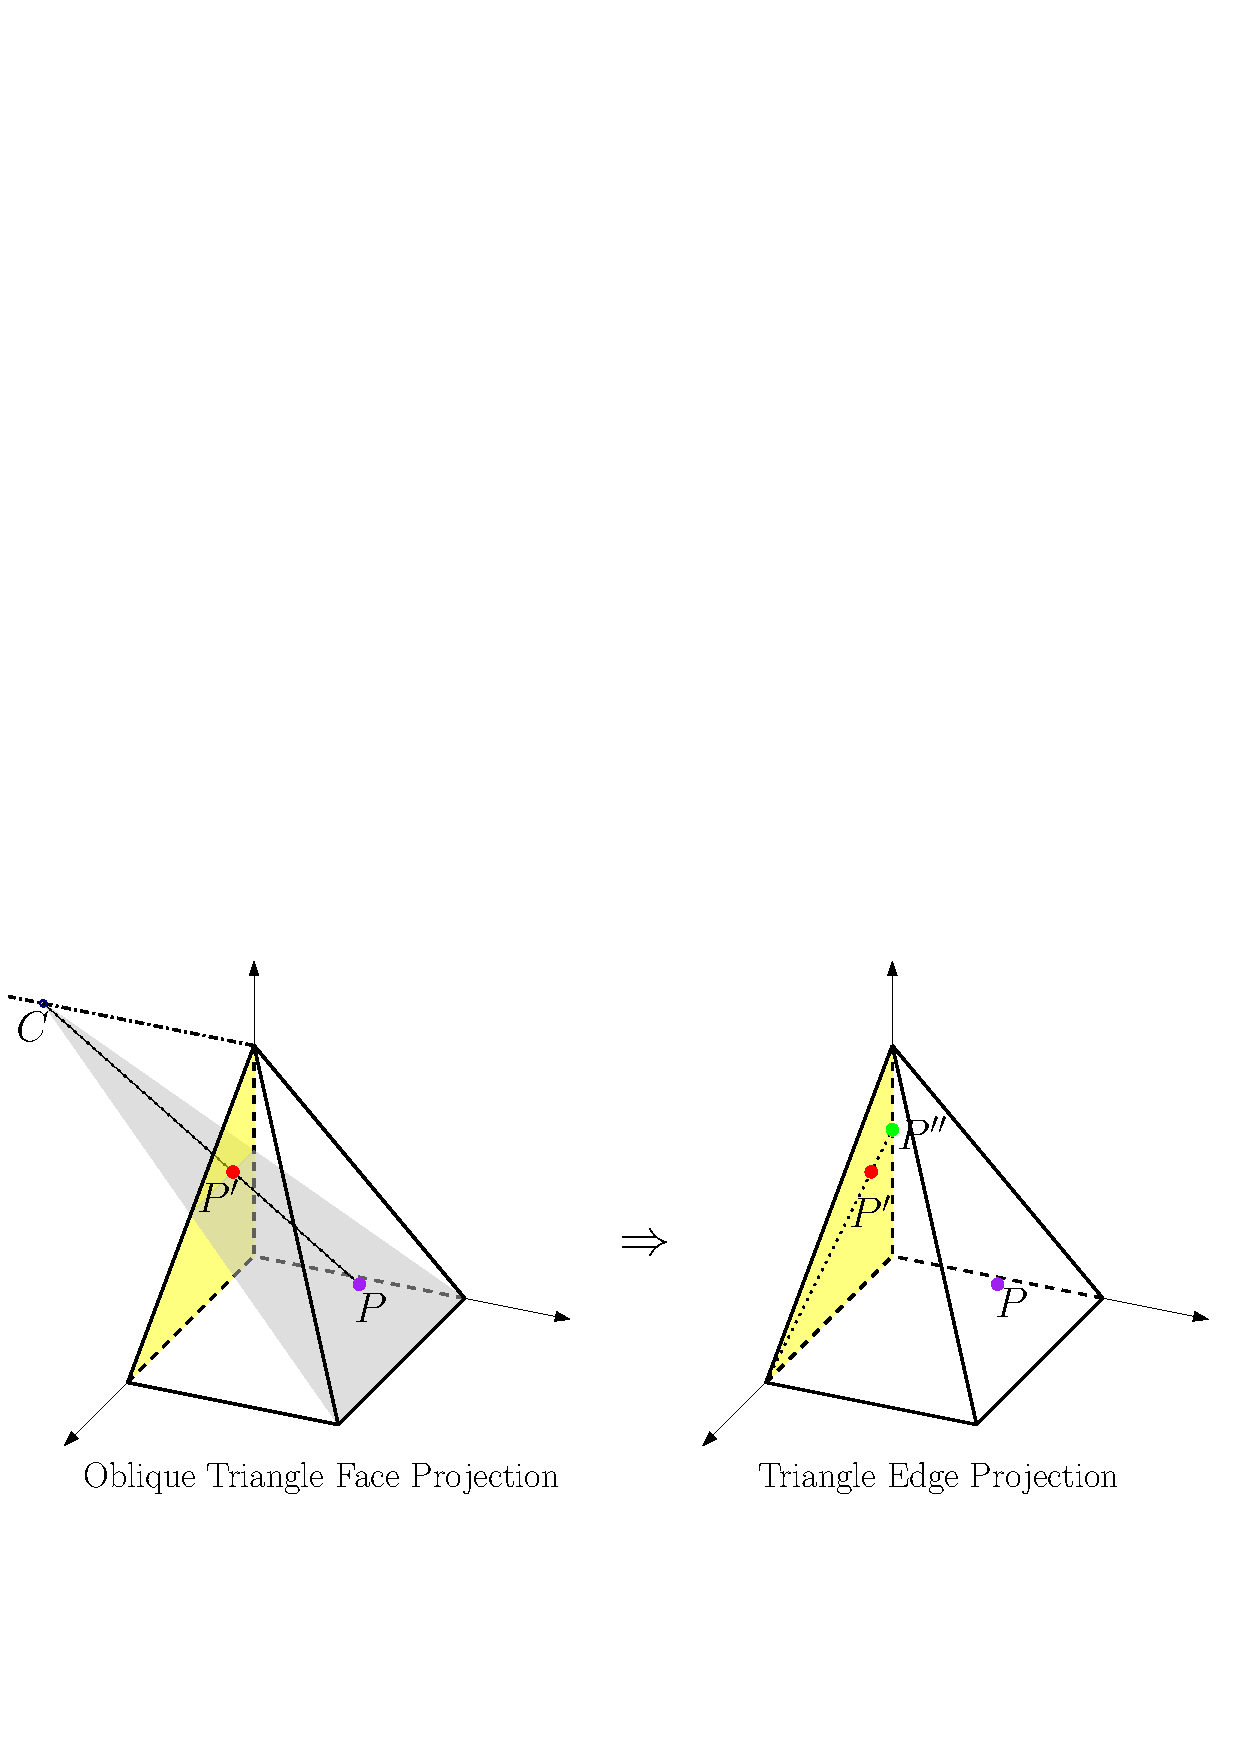
\includegraphics[scale=0.6]{./figures/PyramidProjectionObliqueTriangle.pdf}
\caption{Oblique triangle face projection from $P$ to $P'$ followed by a triangle edge projection from $P'$ to $P''$.}
\label{fig:PyramidProjectionObliqueTriangle}
\end{center}
\end{figure}

In general, the shape functions and their gradient are
\begin{equation}
	\phi_i^\mathrm{e}(\xieta)=\phi_i^\E(\vec{\lambda}_{a5}(\xieta))\,,\qquad\quad
	\nabla\phi_i^\mathrm{e}(\xieta)=\nabla\phi_i^\E(\vec{\lambda}_{a5}(\xieta))\,,
	\label{eq:PyrH1TriaEdge}
\end{equation}
for $i=2,\ldots,p$ and $a=1,2,3,4$.
There are $p-1$ edge functions for each edge, giving a total of $4(p-1)$ triangle edge functions.


\subsubsection{\texorpdfstring{$H^1$}{H1} Faces}

\begin{figure}[!ht]
\begin{center}
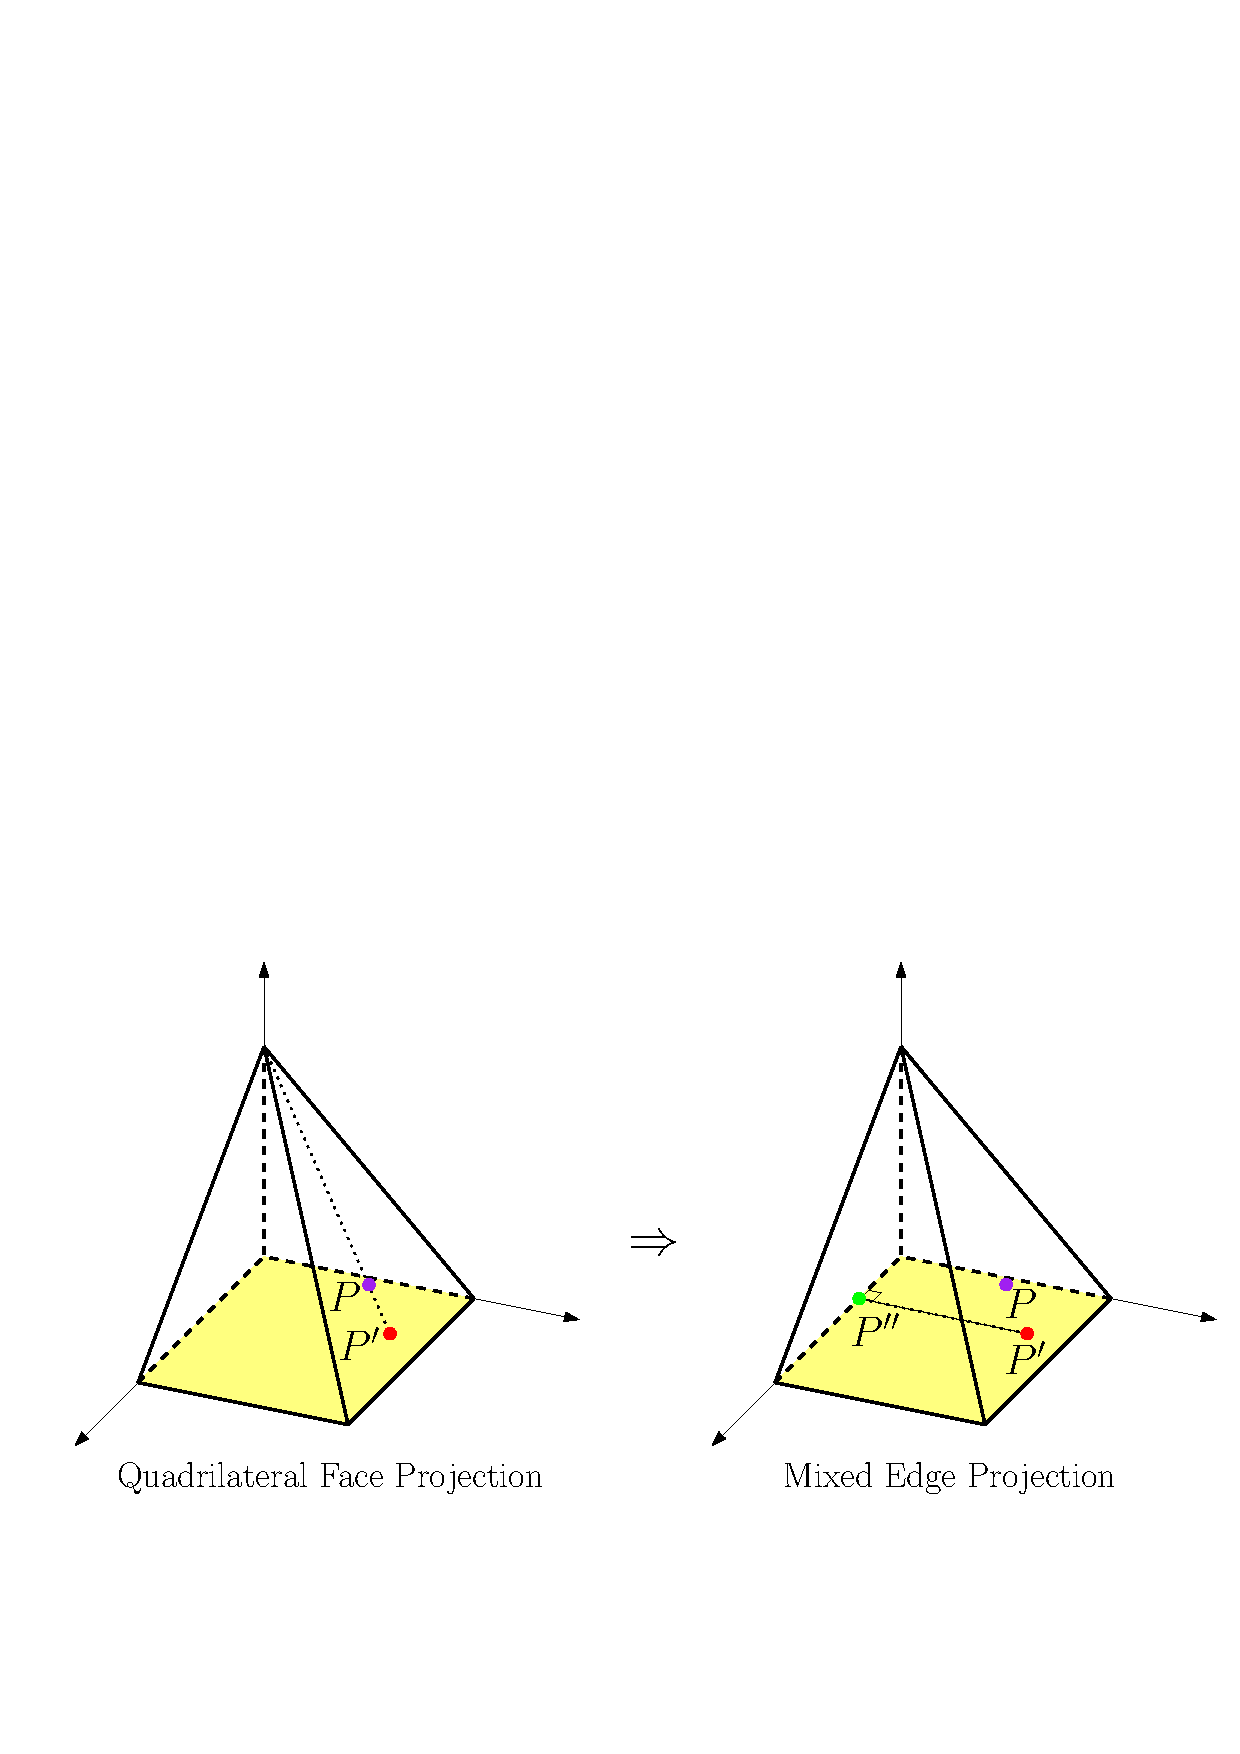
\includegraphics[scale=0.6]{./figures/PyramidProjectionQuad.pdf}
\caption{Quadrilateral face projection from $P$ to $P'$ followed by a mixed edge projection from $P'$ to $P''$.}
\label{fig:PyramidProjectionQuad}
\end{center}
\end{figure}

\paragraph{\texorpdfstring{$H^1$}{H1} Quadrilateral Face.} 
It was already mentioned that the quadrilateral face projection, illustrated in Figure \ref{fig:PyramidProjectionQuad}, takes an arbitrary point $P=(\xi_1,\xi_2,\zeta)$ to the point $P'=(\sxi,\sxii,0)$ along the face. This projected point is actually represented by the affine coordinate quadruple $(\vec{\mu}_{01}(\sxi),\vec{\mu}_{01}(\sxii))$. 
Hence, the natural choice is to use the quadruple with the ancillary function $\phi_{ij}^\square$. 
This already satisfies all the necessary trace properties, except at the top vertex itself, where there might be a singularity.
This is corrected by adding a factor of $\mu_0(\zeta)$, which also ensures the function is in the correct space.

The shape functions and their gradient are
\begin{equation}
	\begin{aligned}
		\phi_{ij}^\mathrm{f}(\xieta)&=\mu_0(\zeta)\phi_{ij}^\square\Big(\vec{\mu}_{01}(\sxi),\vec{\mu}_{01}(\sxii)\Big)\,,\\
    	\nabla\phi_{ij}^\mathrm{f}(\xieta)&=\mu_0(\zeta)\nabla\phi_{ij}^\square\Big(\vec{\mu}_{01}(\sxi),\vec{\mu}_{01}(\sxii)\Big)
        +\phi_{ij}^\square\Big(\vec{\mu}_{01}(\sxi),\vec{\mu}_{01}(\sxii)\Big)\nabla\mu_0(\zeta)\,,	
	\end{aligned}
	\label{eq:PyrH1QuadFace}
\end{equation}
where $i=2,\ldots,p$ and $j=2,\ldots,p$. 
Naturally, there are $(p-1)^2$ shape functions for the quadrilateral face.

\paragraph{\texorpdfstring{$H^1$}{H1} Triangle Faces.} 
Similar to the mixed edges, there are two possibilities.
Obviously they both involve $\phi_{ij}^\Tri$.
Take for example triangle face 125.
The first alternative is to use the 3D pyramid affine coordinates directly, yielding as a result
\begin{equation*}
	\phi_{ij}^\mathrm{f}(\xieta)=\phi_{ij}^\Tri(\vec{\lambda}_{125}(\xieta))=
		\underbrace{(\lambda_1(\xieta)+\lambda_2(\xieta)+\lambda_5(\zeta))^{i+j}}_{\text{blend}}
    	\underbrace{\phi_{ij}^\Tri\Big(\underbrace{\textstyle{\frac{1}{\lambda_1(\xieta)+\lambda_2(\xieta)+\lambda_5(\zeta)}}
    		\vec{\lambda}_{125}(\xieta)}_{\text{project}}\Big)}_{\text{evaluate}}\,,
\end{equation*}
where $i\geq2$ and $j\geq1$.
In this case the projection implied is precisely the oblique triangle face projection illustrated in Figure \ref{fig:PyramidProjectionObliqueTriangle}.
This function lies in the correct space and is easily seen to satisfy the necessary trace properties (see \eqref{eq:phiTrivanishing}).
Hence, it is a perfectly valid candidate.

A second candidate relies in the same approach taken for the mixed edges, in which the effects of the components of $\vec{\lambda}_{12}(\xieta)$ are separated. 
In that case, the functions are
\begin{equation*}
		\phi_{ij}^\mathrm{f}(\xieta)=\underbrace{\mu_0(\sxii)}_{\text{blend}}
    	\underbrace{\phi_{ij}^\Tri\Big(\underbrace{\vec{\nu}_{012}(\xi_1,\zeta)}_{\text{project}}\Big)}_{\text{evaluate}}\,,
\end{equation*}
for $i\geq2$ and $j\geq1$.
Here, the projection implied is the horizontal triangle face projection shown in Figure \ref{fig:PyramidProjectionHorizontalTriangle}.
Again, the function is in the correct space and satisfies the required trace properties, so it is also a valid candidate.

The second alternative is chosen, so the general shape functions and their gradient are
\begin{equation}
	\begin{aligned}
		\phi_{ij}^\mathrm{f}(\xieta)&=\mu_c(\sxib)\phi_{ij}^\Tri(\vec{\nu}_{012}(\xi_a,\zeta))\,,\\
    	\nabla\phi_{ij}^\mathrm{f}(\xieta)&=\mu_c(\sxib)\nabla\phi_{ij}^\Tri(\vec{\nu}_{012}(\xi_a,\zeta))
        +\phi_{ij}^\Tri(\vec{\nu}_{012}(\xi_a,\zeta))\nabla\mu_c(\sxib)\,,	
	\end{aligned}
	\label{eq:PyrH1TriaFace}
\end{equation}
where $i\geq2$, $j\geq1$, $n=i+j=3,\ldots,p$, $(a,b)=(1,2),(2,1)$ and $c=0,1$.
As with all $H^1$ triangle edges, there are $\frac{1}{2}(p-1)(p-2)$ face functions for each face, for a total of $2(p-1)(p-2)$ triangle face functions.

\subsubsection{\texorpdfstring{$H^1$}{H1} Interior Bubbles}

The interior bubble functions resemble closely the case of the hexahedron bubbles, and they are deduced from the quadrilateral face functions, where the factor $\phi_k^\E(\vec{\mu}_{01}(\zeta))$ is used instead of $\mu_0(\zeta)$.
This ensures all the vanishing properties are satisfied.

The bubble functions and their gradient are
\begin{equation}
	\begin{aligned}
		\phi_{ijk}^\mathrm{b}(\xieta)&\!=\!
			\phi_{ij}^\square\Big(\vec{\mu}_{01}(\sxi),\vec{\mu}_{01}(\sxii)\Big)\phi_k^\E(\vec{\mu}_{01}(\zeta))\,,\\
    		\nabla\phi_{ijk}^\mathrm{b}(\xieta)&\!=\!\phi_k^\E(\vec{\mu}_{01}(\zeta))
    			\nabla\phi_{ij}^\square\Big(\vec{\mu}_{01}(\sxi),\vec{\mu}_{01}(\sxii)\Big)
        		\!+\!\phi_{ij}^\square\Big(\vec{\mu}_{01}(\sxi),\vec{\mu}_{01}(\sxii)\Big)\nabla\phi_k^\E(\vec{\mu}_{01}(\zeta))\,,	
	\end{aligned}
	\label{eq:PyrH1Interior}
\end{equation}
where $i=2,\ldots,p$, $j=2,\ldots,p$ and $k=2,\ldots,p$.
Clearly there is a total of $(p-1)^3$ interior bubble functions.

\subsection{\texorpdfstring{$H(\mathrm{curl})$}{Hcurl} Shape Functions}

The dimension of the space $\mathcal{U}^{(1),p}$ is $3p^3+5p$.
The same number of shape functions will span the space.

The construction of the shape functions for $H(\mathrm{curl})$ is completely parallel to that of $H^1$, and they involve the same underlying projections.

\subsubsection{\texorpdfstring{$H(\mathrm{curl})$}{Hcurl} Edges}

\paragraph{\texorpdfstring{$H(\mathrm{curl})$}{Hcurl} Mixed Edges.} 
Take for example mixed edge 12.
As in $H^1$, using $\mu_0(\sxii)$ and $\vec{\nu}_{01}(\xi_1,\zeta)$ separately instead of $\vec{\lambda}_{12}(\xieta)$, it follows the edge shape functions are
\begin{equation*}
	E_i^\mathrm{e}(\xieta)=\mu_0(\sxii)E_i^\E(\vec{\nu}_{01}(\xi_1,\zeta))=
		\underbrace{\mu_0(\sxii)(\nu_0(\xi_1,\zeta)\!+\!\nu_1(\xi_1,\zeta))^{i+2}}_{\text{blend}}
    	\underbrace{E_i^\E\Big(\underbrace{\textstyle{\frac{1}{\nu_0(\xi_1,\zeta)+\nu_1(\xi_1,\zeta)}}
    		\vec{\nu}_{01}(\xi_1,\zeta)}_{\text{project}}\Big)}_{\text{evaluate}}\,,
\end{equation*}
for $i=0,\ldots,p-1$.
From the $H(\mathrm{curl})$ edge triangle functions, it follows that along the edges 15 and 25 the tangential component of $E_i^\E(\vec{\nu}_{01}(\xi_1,\zeta))$ vanishes, and due to its independence from $\xi_2$ it immediately follows that the same is true for the faces 235 and 145.
Along face 435, it holds that $\mu_0(\sxii)=0$ so that it also vanishes there.
Along face 125 $\mu_0(\sxii)=1$, and the function becomes $E_i^\E(\vec{\nu}_{01}(\xi_1,\zeta))$, which as desired is the triangle 2D trace for the edge functions.
Finally, at the quadrilateral face, $\mu_0(\sxii)=\mu_0(\xi_2)$, while the tangential component of $E_i^\E(\vec{\nu}_{01}(\xi_1,\zeta))$ is the corresponding segment 1D $L^2$ edge function, meaning that the trace along this face is $\mu_0(\xi_2)E_i^\E(\vec{\mu}_{01}(\xi_1))$, as required.
Hence, all trace properties hold.
The projection implied is the mixed edge projection depicted in Figures \ref{fig:PyramidProjectionHorizontalTriangle} and \ref{fig:PyramidProjectionQuad}.
Lastly, the shape functions are in the correct space.

The shape functions and their curl are
\begin{equation}
	\begin{aligned}
		E_i^\mathrm{e}(\xieta)&=\mu_c(\sxib)E_i^\E(\vec{\nu}_{01}(\xi_a,\zeta))\,,\\
    	\nabla\times E_i^\mathrm{e}(\xieta)&=\mu_c(\sxib)\nabla\times E_i^\E(\vec{\nu}_{01}(\xi_a,\zeta))
        +\nabla\mu_c(\sxib)\times E_i^\E(\vec{\nu}_{01}(\xi_a,\zeta))\,,	
	\end{aligned}
	\label{eq:PyrHcurlMixedEdge}
\end{equation}
where $i=0,\ldots,p-1$, $(a,b)=(1,2),(2,1)$ and $c=0,1$.
There are $p$ edge functions for each edge, for a total of $4p$ mixed edge functions.

\paragraph{\texorpdfstring{$H(\mathrm{curl})$}{Hcurl} Triangle Edges.}
For instance, take triangle edge 15.
Like in $H^1$, one can directly use the 3D pyramid affine coordinates on $E_i^\E$.
The resulting shape functions are
\begin{equation*}
	E^\mathrm{e}(\xieta)=E_i^\E(\vec{\lambda}_{15}(\xieta))=
		\underbrace{(\lambda_1(\xieta)+\lambda_5(\zeta))^{i+2}}_{\text{blend}}
    	\underbrace{E_i^\E\Big(\underbrace{\textstyle{\frac{1}{\lambda_1(\xieta)+\lambda_5(\zeta)}}
    		\vec{\lambda}_{15}(\xieta)}_{\text{project}}\Big)}_{\text{evaluate}}\,,
\end{equation*}
for $i=0,\ldots,p-1$.
To argue the nonzero traces have the correct form, take for example face 125, and the decoupling $\lambda_1(\xieta)=\mu_0(\sxii)\nu_0(\xi_1,\zeta)$.
Then, using that $\nu_2(\zeta)=\lambda_5(\zeta)$, the lowest order element is
\begin{equation*}
\begin{aligned}
	E_0^\E(\vec{\lambda}_{15}(\xieta))
		&=\mu_0(\sxii)\nu_0(\xi_1,\zeta)\nabla\lambda_5(\zeta)-\lambda_5(\zeta)\nabla\Big(\mu_0(\sxii)\nu_0(\xi_1,\zeta)\Big)\\
			&=\mu_0(\sxii)E_0^\E(\vec{\nu}_{02}(\xi_1,\zeta))-\nu_0(\xi_1,\zeta)\nu_2(\zeta)\nabla\mu_0(\sxii)\,.
\end{aligned}
\end{equation*}
When evaluated at face 125, $\mu_0(\sxii)=1$, and as a result $\nabla\mu_0(\sxii)$ is orthogonal to the face (it is an isosurface), so that the tangential component at the face is precisely the nonzero components of $E_0^\E(\vec{\nu}_{02}(\xi_1,\zeta))$.
Hence, its nonzero trace on the face is a triangle 2D $H(\mathrm{curl})$ edge function, as expected.
Using the same argument but at face 435, where $\mu_0(\sxii)=0$, this time the tangential component vanishes completely.  
Symmetric arguments apply to faces 145 and 235.
Finally, at the quadrilateral face, where $\lambda_5(\zeta)=0$, the lowest order function takes the form $\lambda_1(\xieta)\nabla\lambda_5(\zeta)$ which is normal to the face (it is an isosurface of $\lambda_5(\zeta)$), so the tangential component is zero.
These arguments confirm that the trace properties hold.
Lastly, the projection is a triangle edge projection as illustrated in Figure \ref{fig:PyramidProjectionObliqueTriangle}.

The shape functions and their curl are
\begin{equation}
	E_i^\mathrm{e}(\xieta)=E_i^\E(\vec{\lambda}_{a5}(\xieta))\,,\qquad\quad
	\nabla\times E_i^\mathrm{e}(\xieta)=\nabla \times E_i^\E(\vec{\lambda}_{a5}(\xieta))\,,
	\label{eq:PyrHcurlTriaEdge}
\end{equation}
for $i=0,\ldots,p-1$ and $a=1,2,3,4$.
There are $p$ edge functions for each edge, for a total of $4p$ triangle edge functions.

\subsubsection{\texorpdfstring{$H(\mathrm{curl})$}{Hcurl} Faces}

\paragraph{\texorpdfstring{$H(\mathrm{curl})$}{Hcurl} Quadrilateral Face.} 
As expected, the projection implied in these expressions will be the same as that of $H^1$. 
It is a quadrilateral face projection as depicted in Figure \ref{fig:PyramidProjectionQuad}.
However, in this case there will be two families.
Both families will easily satisfy the vanishing trace properties by use of \eqref{eq:phiEvanishing}, \eqref{eq:Hcurl1Dspecialcase} and that $\nabla\mu_c(\sxia)$ is orthogonal to the triangle faces where $\mu_c(\sxia)=1$.
The only difference with $H^1$ radicates in the use of the higher order blending function $\mu_0(\zeta)^2$, which is used in order to be in the correct space. 
There is a grand total of $2p(p-1)$ quadrilateral face functions.

\subparagraph{Family I:}
The shape functions and their curl are
\begin{equation}
	\begin{aligned}
		E_{ij}^{\mathrm{f}}(\xieta)&=\mu_0(\zeta)^2 E_{ij}^\square\Big(\vec{\mu}_{01}(\sxi),\vec{\mu}_{01}(\sxii)\Big)\,,\\
		\nabla\times E_{ij}^{\mathrm{f}}(\xieta)&=\mu_0(\zeta)^2\nabla\times
			E_{ij}^\square\Big(\vec{\mu}_{01}(\sxi),\vec{\mu}_{01}(\sxii)\Big)\\
				&\qquad\quad+2\mu_0(\zeta)\nabla\mu_0(\zeta)\times E_{ij}^\square\Big(\vec{\mu}_{01}(\sxi),\vec{\mu}_{01}(\sxii)\Big)\,,
	\end{aligned}
	\label{eq:PyrHcurlQuadFaceI}
\end{equation}
for $i=0,\ldots,p-1$ and $j=2,\ldots,p$. 
There are $p(p-1)$ shape functions in this family.

\subparagraph{Family II:}
The shape functions and their curl are
\begin{equation}
	\begin{aligned}
		E_{ij}^{\mathrm{f}}(\xieta)&=\mu_0(\zeta)^2 E_{ij}^\square\Big(\vec{\mu}_{01}(\sxii),\vec{\mu}_{01}(\sxi)\Big)\,,\\
		\nabla\times E_{ij}^{\mathrm{f}}(\xieta)&=\mu_0(\zeta)^2\nabla\times
			E_{ij}^\square\Big(\vec{\mu}_{01}(\sxii),\vec{\mu}_{01}(\sxi)\Big)\\
				&\qquad\quad+2\mu_0(\zeta)\nabla\mu_0(\zeta)\times E_{ij}^\square\Big(\vec{\mu}_{01}(\sxii),\vec{\mu}_{01}(\sxi)\Big)\,,
	\end{aligned}
	\label{eq:PyrHcurlQuadFaceII}
\end{equation}
for $i=0,\ldots,p-1$ and $j=2,\ldots,p$. 
Note the fact that the entries are permuted with respect to the first family.
There are $p(p-1)$ shape functions in this family.

\paragraph{\texorpdfstring{$H(\mathrm{curl})$}{Hcurl} Triangle Faces.} 
As with $H^1$ there will be two valid alternatives.
Take for example face 125.
The first alternative is to use the pyramid affine coordinates directly on $E_{ij}^\Tri$ \textit{and} multiply by $\mu_0(\sxii)^{-1}$.
This approach is discarded in favor of separating the effects of $\mu_0(\sxii)$ and $\vec{\nu}_{01}(\xi_1,\zeta)$ directly from $\vec{\lambda}_{12}(\xieta)$.
The resulting functions satisfy the necessary vanishing conditions using similar arguments to those used for mixed and triangle edges.
Also, the projection implied is the horizontal triangle face projection shown in Figure \ref{fig:PyramidProjectionHorizontalTriangle}.
There are $p(p-1)$ functions per triangle face, for a grand total of $4p(p-1)$ triangle face functions.

\subparagraph{Family I:} 
The shape functions and their curl are
\begin{equation}
	\begin{aligned}
		E_{ij}^{\mathrm{f}}(\xieta)&=\mu_c(\sxib)E_{ij}^\Tri(\vec{\nu}_{012}(\xi_a,\zeta))\,,\\
		\nabla\times E_{ij}^{\mathrm{f}}(\xieta)&=\mu_c(\sxib)\nabla\times E_{ij}^\Tri(\vec{\nu}_{012}(\xi_a,\zeta))
			+\nabla\mu_c(\sxib)\times E_{ij}^\Tri(\vec{\nu}_{012}(\xi_a,\zeta))\,,
	\end{aligned}
	\label{eq:PyrHcurlTriaFaceI}
\end{equation}
for $i\geq0$, $j\geq1$, $n=i+j=1,\ldots,p-1$, $(a,b)=(1,2),(2,1)$, and $c=0,1$. 
Every face has $\frac{1}{2}p(p-1)$ functions in this family.

\subparagraph{Family II:} 
The shape functions and their curl are
\begin{equation}
	\begin{aligned}
		E_{ij}^{\mathrm{f}}(\xieta)&=\mu_c(\sxib)E_{ij}^\Tri(\vec{\nu}_{120}(\xi_a,\zeta))\,,\\
		\nabla\times E_{ij}^{\mathrm{f}}(\xieta)&=\mu_c(\sxib)\nabla\times E_{ij}^\Tri(\vec{\nu}_{120}(\xi_a,\zeta))
			+\nabla\mu_c(\sxib)\times E_{ij}^\Tri(\vec{\nu}_{120}(\xi_a,\zeta))\,,
	\end{aligned}
	\label{eq:PyrHcurlTriaFaceII}
\end{equation}
for $i\geq0$, $j\geq1$, $n=i+j=1,\ldots,p-1$, $(a,b)=(1,2),(2,1)$, and $c=0,1$. 
Note the fact that the entries are $\vec{\nu}_{120}(\xi_a,\zeta)$ as opposed to $\vec{\nu}_{012}(\xi_a,\zeta)$.
Every face has $\frac{1}{2}p(p-1)$ functions in this family.

\subsubsection{\texorpdfstring{$H(\mathrm{curl})$}{Hcurl} Interior Bubbles}

These will be separated according to a Helmholtz decomposition.
Indeed, there are four families of interior bubbles, and the first family corresponds precisely to the gradients of $H^1$ interior bubble functions, so they have zero curl.
The other three families will essentially be generated by quadrilateral face functions in $H(\mathrm{curl})$ and $H^1$.
In all cases, the trace properties follow easily.
There is a grand total of $3p(p-1)^2$ interior bubble functions.

\subparagraph{Family I:}
These are the gradients of $H^1$ interior functions.
The shape functions and their curl are
\begin{equation}
	\begin{aligned}
		E_{ijk}^\mathrm{b}(\xieta)&=\phi_k^\E(\vec{\mu}_{01}(\zeta))
    			\nabla\phi_{ij}^\square\Big(\vec{\mu}_{01}(\sxi),\vec{\mu}_{01}(\sxii)\Big)\\
        		&\quad\qquad+\phi_{ij}^\square\Big(\vec{\mu}_{01}(\sxi),\vec{\mu}_{01}(\sxii)\Big)\nabla\phi_k^\E(\vec{\mu}_{01}(\zeta))\,,\\
    \nabla\times E_{ijk}^\mathrm{b}(\xieta)&=0\,,
	\end{aligned}
	\label{eq:PyrHcurlInteriorI}
\end{equation}
where $i=2,\ldots,p$, $j=2,\ldots,p$ and $k=2,\ldots,p$.
There are $(p-1)^3$ interior bubble functions in this family.

\subparagraph{Family II:}
The shape functions and their curl are
\begin{equation}
	\begin{aligned}
		E_{ijk}^{\mathrm{b}}(\xieta)&=\mu_0(\zeta)\phi_k^\E(\vec{\mu}_{01}(\zeta))
			E_{ij}^\square\Big(\vec{\mu}_{01}(\sxi),\vec{\mu}_{01}(\sxii)\Big)\,,\\
		\nabla\times E_{ijk}^{\mathrm{b}}(\xieta)&=\mu_0(\zeta)\phi_k^\E(\vec{\mu}_{01}(\zeta))\nabla\times
			E_{ij}^\square\Big(\vec{\mu}_{01}(\sxi),\vec{\mu}_{01}(\sxii)\Big)\\
				&\quad+\Big(\mu_0(\zeta)\nabla\phi_k^\E(\vec{\mu}_{01}(\zeta))+\phi_k^\E(\vec{\mu}_{01}(\zeta))\nabla\mu_0(\zeta)\Big)
					\times E_{ij}^\square\Big(\vec{\mu}_{01}(\sxi),\vec{\mu}_{01}(\sxii)\Big)\,,
	\end{aligned}
	\label{eq:PyrHcurlInteriorII}
\end{equation}
for $i=0,\ldots,p-1$, $j=2,\ldots,p$, and $k=2,\ldots,p$.
There are $p(p-1)^2$ shape functions in this family.

\subparagraph{Family III:}
The shape functions and their curl are
\begin{equation}
	\begin{aligned}
		E_{ijk}^{\mathrm{b}}(\xieta)&=\mu_0(\zeta)\phi_k^\E(\vec{\mu}_{01}(\zeta))
			E_{ij}^\square\Big(\vec{\mu}_{01}(\sxii),\vec{\mu}_{01}(\sxi)\Big)\,,\\
		\nabla\times E_{ijk}^{\mathrm{b}}(\xieta)&=\mu_0(\zeta)\phi_k^\E(\vec{\mu}_{01}(\zeta))\nabla\times
			E_{ij}^\square\Big(\vec{\mu}_{01}(\sxii),\vec{\mu}_{01}(\sxi)\Big)\\
				&\quad+\Big(\mu_0(\zeta)\nabla\phi_k^\E(\vec{\mu}_{01}(\zeta))+\phi_k^\E(\vec{\mu}_{01}(\zeta))\nabla\mu_0(\zeta)\Big)
					\times E_{ij}^\square\Big(\vec{\mu}_{01}(\sxii),\vec{\mu}_{01}(\sxi)\Big)\,,
	\end{aligned}
	\label{eq:PyrHcurlInteriorIII}
\end{equation}
for $i=0,\ldots,p-1$, $j=2,\ldots,p$, and $k=2,\ldots,p$.
Note the entries are permuted with respect to the second family of interior bubbles.
There are $p(p-1)^2$ shape functions in this family.

\subparagraph{Family IV:}
The shape functions for the final family of interior bubbles and their curl are
\begin{equation}
	\begin{aligned}
		E_{ij}^{\mathrm{b}}(\xieta)&=\phi_{ij}^\square\Big(\vec{\mu}_{01}(\sxii),\vec{\mu}_{01}(\sxi)\Big)
			n\mu_0(\zeta)^{n-1}\nabla\mu_0(\zeta)\,,\\
		\nabla\times E_{ij}^{\mathrm{b}}(\xieta)&=n\mu_0(\zeta)^{n-1}
			\nabla\phi_{ij}^\square\Big(\vec{\mu}_{01}(\sxii),\vec{\mu}_{01}(\sxi)\Big)\times\nabla\mu_0(\zeta)\,,
	\end{aligned}
	\label{eq:PyrHcurlInteriorIV}
\end{equation}
for $i=2,\ldots,p$, $j=2,\ldots,p$, and $n=\max\{i,j\}$.
There are $(p-1)^2$ shape functions in this family.


\subsection{\texorpdfstring{$H(\mathrm{div})$}{Hdiv} Shape Functions}

The dimension of the space $\mathcal{U}^{(2),p}$ is $3p^3+2p$.
The number of linearly independent shape functions coincides with that dimension.

\subsubsection{\texorpdfstring{$H(\mathrm{div})$}{Hdiv} Faces}

\paragraph{\texorpdfstring{$H(\mathrm{div})$}{Hdiv} Quadrilateral Face.} 
These are constructed exactly the same way as the $H^1$ and $H(\mathrm{curl})$ counterparts, but with the higher order blending function $\mu_0(\zeta)^3$ so that the resulting functions lie in the space.
In view of \eqref{eq:Vijsimplified}, it is clear that the function will only have a tangential component along the triangle faces, so that the normal trace vanishes at these faces, as required.
Moreover, again through \eqref{eq:Vijsimplified}, it is evident that the nonzero trace on the face is a quadrilateral $L^2$ face function.
The projection is once again depicted in Figure \ref{fig:PyramidProjectionQuad}.

In view of \eqref{eq:Vijsimplified}, the shape functions and their divergence are
\begin{equation}
	\begin{aligned}
		V_{ij}^\mathrm{f}(\xieta)&=\mu_0(\zeta)^3V_{ij}^\square\Big(\vec{\mu}_{01}(\sxi),\vec{\mu}_{01}(\sxii)\Big)\,,\\
    	\nabla\cdot V_{ij}^\mathrm{f}(\xieta)&=3\mu_0(\zeta)^2\nabla\mu_0(\zeta)\cdot
    		V_{ij}^\square\Big(\vec{\mu}_{01}(\sxi),\vec{\mu}_{01}(\sxii)\Big)\,,	
	\end{aligned}
	\label{eq:PyrHdivQuadFace}
\end{equation}
where $i=0,\ldots,p-1$ and $j=0,\ldots,p-1$.
Clearly, there are $p^2$ quadrilateral face functions.

\paragraph{\texorpdfstring{$H(\mathrm{div})$}{Hdiv} Triangle Faces.} 
The construction of the $H(\mathrm{div})$ triangle face functions is highly nontrivial.
Indeed, an analogous construction to the case of $H^1$ or $H(\mathrm{curl})$ does not work here.
This radicates in the definition of the space itself.
The issue is even present for the lowest order space, and in fact it is by looking at this space in detail that the problem is solved.

To summarize the construction, take for example face 125.
The detailed calculations are in Appendix \ref{app:pyrappendix}.
Proceeding as in the $H^1$ or $H(\mathrm{curl})$ case, one obtains the following two disheartening facts for the lowest order candidate functions,
\begin{equation*}
	\mu_0\big(\sxii\big)V_{00}^\Tri(\vec{\nu}_{012}(\xi_1,\zeta))\notin\mathcal{U}^{(2),1}\,,\qquad\quad
	\mu_0\big(\sxii\big)^{-1}V_{00}^\Tri(\vec{\lambda}_{125}(\xieta))\notin\mathcal{U}^{(2),1}\,.
\end{equation*}
However, they both satisfy the desired trace properties.
One could alternatively attempt a more direct construction, but issues arise constantly, either because the functions are not in the space, or because there are ``illegal'' derivatives of Legendre polynomials $P_i$, which in theory should not exist as they are elements of $L^2$ and are intended to approximate elements of that space (for example, a discontinuous function).
These issues do not arise when using $V_{ij}^\Tri$ in view of Lemma \ref{lem:divformula}, and this is one of the reasons why it is so convenient to use it.
Fortunately, there is a way to make this happen.
The key is to look at the unique lowest order function for a given face. 
The explicit formulas are given in \citet{Hiptmair99} and \citet{Nigam_Phillips_11}.
After scrupulous observation, one obtains
\begin{equation*}
	V_{00}^\mathrm{f}(\xieta)=\frac{1}{2}\Big(\mu_0\big(\sxii\big)V_{00}^\Tri(\vec{\nu}_{012}(\xi_1,\zeta))+
		\mu_0\big(\sxii\big)^{-1}V_{00}^\Tri(\vec{\lambda}_{125}(\xieta))\Big)\in\mathcal{U}^{(2),1}\,.
\end{equation*}
Hence, this suggests the following general formula for the face 125 shape functions,
\begin{equation*}
	V_{ij}^\mathrm{f}(\xieta)=\frac{1}{2}\Big(\mu_0\big(\sxii\big)V_{ij}^\Tri(\vec{\nu}_{012}(\xi_1,\zeta))+
		\mu_0\big(\sxii\big)^{-1}V_{ij}^\Tri(\vec{\lambda}_{125}(\xieta))\Big)\,,
\end{equation*}
for $i\geq0$, $j\geq0$, and $n=i+j=0,\ldots,p-1$. 
In Appendix \ref{app:pyrappendix} it is shown that these high order functions are in the correct space and that they sastisfy the trace properties.
%The trace properties are inherited from each of the separate terms, and they hold as well (see Appendix \ref{app:pyrappendix}).
Some could worry when seeing the factor $\mu_0\big(\sxii\big)^{-1}$, but this is in fact not a real singularity.
Indeed it is shown in Appendix \ref{app:pyrappendix} how to avoid it explicitly, along with an alternative formula convenient for computations.
Lastly, note the inherent projection is not unique, and in fact is a combination of horizontal and oblique triangle face projections.

Finally, in view of \eqref{eq:HdivtriangleRemark} the general shape functions are 
\begin{equation}
	\begin{aligned}
		V_{ij}^\mathrm{f}(\xieta)&=\frac{1}{2}\Big(\mu_c\big(\sxib\big)V_{ij}^\Tri(\vec{\nu}_{012}(\xi_a,\zeta))
			+\mu_c\big(\sxib\big)^{-1}V_{ij}^\Tri(\vec{\lambda}_{de5}(\xieta))\Big)\,,\\
    \nabla\cdot V_{ij}^\mathrm{f}(\xieta)&=\frac{1}{2}\Big(\nabla\mu_c\big(\sxib\big)\cdot V_{ij}^\Tri(\vec{\nu}_{012}(\xi_a,\zeta))
    	+\mu_c\big(\sxib\big)^{-1}\nabla\cdot V_{ij}^\Tri(\vec{\lambda}_{de5}(\xieta))\\
    		&\qquad\qquad\qquad\qquad\qquad\qquad\quad
    			-\mu_c\big(\sxib\big)^{-2}\nabla\mu_c(\sxib)\cdot V_{ij}^\Tri(\vec{\lambda}_{de5}(\xieta))\Big)\,,	
	\end{aligned}
	\label{eq:PyrHdivTriaFace}
\end{equation}
where $i\geq0$, $j\geq0$, $n=i+j=0,\ldots,p-1$, $(a,b)=(1,2),(2,1)$, $c=0,1$ and where $(d,e)$ depends on $(a,b,c)$ (in fact $\vec{\lambda}_{de5}(\xieta)=\mu_c\big(\sxib\big)\vec{\nu}_{012}(\xi_a,\zeta)$).
%$(a,b,c,d,e)=(1,2,0,1,2),(2,1,1,2,3),(1,2,1,4,3),(2,1,0,1,4)$.
There are $\frac{1}{2}p(p+1)$ functions for each face, leading to a total of $2p(p-1)$ triangle face functions.

\subsubsection{\texorpdfstring{$H(\mathrm{div})$}{Hdiv} Interior Bubbles}

Like the $H(\mathrm{curl})$ interior bubbles, these will be separated according to a Helmholtz decomposition.
Indeed, the first three out of seven families of interior bubbles are precisely the curl of $H(\mathrm{curl})$ interior bubble functions, so they have zero divergence.
In all cases, the trace properties follow easily.
There is a grand total of $3p^2(p-1)$ interior bubble functions.

\subparagraph{Family I:}
The shape functions and their divergence are
\begin{equation}
	\begin{aligned}
		V_{ijk}^{\mathrm{b}}(\xieta)&=\mu_0(\zeta)\phi_k^\E(\vec{\mu}_{01}(\zeta))\nabla\times
			E_{ij}^\square\Big(\vec{\mu}_{01}(\sxi),\vec{\mu}_{01}(\sxii)\Big)\\
				&\quad+\Big(\mu_0(\zeta)\nabla\phi_k^\E(\vec{\mu}_{01}(\zeta))+\phi_k^\E(\vec{\mu}_{01}(\zeta))\nabla\mu_0(\zeta)\Big)
					\times E_{ij}^\square\Big(\vec{\mu}_{01}(\sxi),\vec{\mu}_{01}(\sxii)\Big)\,,\\
		\nabla\cdot V_{ijk}^{\mathrm{b}}(\xieta)&=0\,,
	\end{aligned}
	\label{eq:PyrHdivInteriorI}
\end{equation}
for $i=0,\ldots,p-1$, $j=2,\ldots,p$, and $k=2,\ldots,p$.
There are $p(p-1)^2$ shape functions in this family.

\subparagraph{Family II:}
The shape functions and their divergence are
\begin{equation}
	\begin{aligned}
		V_{ijk}^{\mathrm{b}}(\xieta)&=\mu_0(\zeta)\phi_k^\E(\vec{\mu}_{01}(\zeta))\nabla\times
			E_{ij}^\square\Big(\vec{\mu}_{01}(\sxii),\vec{\mu}_{01}(\sxi)\Big)\\
				&\quad+\Big(\mu_0(\zeta)\nabla\phi_k^\E(\vec{\mu}_{01}(\zeta))+\phi_k^\E(\vec{\mu}_{01}(\zeta))\nabla\mu_0(\zeta)\Big)
					\times E_{ij}^\square\Big(\vec{\mu}_{01}(\sxii),\vec{\mu}_{01}(\sxi)\Big)\,,\\
		\nabla\cdot V_{ijk}^{\mathrm{b}}(\xieta)&=0\,,
	\end{aligned}
	\label{eq:PyrHdivInteriorII}
\end{equation}
for $i=0,\ldots,p-1$, $j=2,\ldots,p$, and $k=2,\ldots,p$.
Note the entries are permuted with respect to the first family of interior bubbles.
There are $p(p-1)^2$ shape functions in this family.

\subparagraph{Family III:}
The shape functions and their divergence are
\begin{equation}
	\begin{aligned}
		V_{ij}^{\mathrm{b}}(\xieta)&=n\mu_0(\zeta)^{n-1}
			\nabla\phi_{ij}^\square\Big(\vec{\mu}_{01}(\sxii),\vec{\mu}_{01}(\sxi)\Big)\times\nabla\mu_0(\zeta)\,,\\
		\nabla\cdot V_{ij}^{\mathrm{b}}(\xieta)&=0\,,
	\end{aligned}
	\label{eq:PyrHdivInteriorIII}
\end{equation}
for $i=2,\ldots,p$, $j=2,\ldots,p$, and $n=\max\{i,j\}$.
There are $(p-1)^2$ shape functions in this family.

\subparagraph{Family IV:}
These have nonzero divergence and are generated by the quadrilateral face functions, but using $\mu_0(\zeta)^2\phi_k^\E(\vec{\mu}_{01}(\zeta))$ as a factor instead of $\mu_0(\zeta)^3$. 
In view of \eqref{eq:Vijsimplified}, the shape functions and their divergence are
\begin{equation}
	\begin{aligned}
		V_{ijk}^{\mathrm{b}}(\xieta)&\!=\!\mu_0(\zeta)^2\phi_k^\E(\vec{\mu}_{01}(\zeta))
			V_{ij}^\square\Big(\vec{\mu}_{01}(\sxi),\vec{\mu}_{01}(\sxii)\Big)\,,\\
		\nabla\!\cdot\! V_{ijk}^{\mathrm{b}}(\xieta)&\!=\!
				\Big(\mu_0(\zeta)^2\nabla\phi_k^\E(\vec{\mu}_{01}(\zeta))
					\!+\!2\mu_0(\zeta)\phi_k^\E(\vec{\mu}_{01}(\zeta))\nabla\mu_0(\zeta)\Big)
						\!\cdot\! V_{ij}^\square\Big(\vec{\mu}_{01}(\sxi),\vec{\mu}_{01}(\sxii)\Big)\,,
	\end{aligned}
	\label{eq:PyrHdivInteriorIV}
\end{equation}
for $i=0,\ldots,p-1$, $j=0,\ldots,p-1$, and $k=2,\ldots,p$.
There are $p^2(p-1)$ shape functions in this family.

\subparagraph{Family V:}
These have nonzero divergence and are expressed as the product of a power of $\mu_1(\zeta)$ with a curl. 
As a first step, define
\begin{equation}
\begin{aligned}
		V_{ij}^\trianglelefteq(\vec{s}_{01}^{\,x},\vec{s}_{01}^{\,y},t_0)&\!=\!\nabla\!\times\!\Big(\textstyle{\frac{1}{2}}t_0^2
			\Big(\phi_i^\E(\vec{s}_{01}^{\,x})\nabla\phi_j^\E(\vec{s}_{01}^{\,y})
					\!-\!\phi_j^\E(\vec{s}_{01}^{\,y})\nabla\phi_i^\E(\vec{s}_{01}^{\,x})\Big)\Big)\,,\\
			&\!=\!t_0^2\Big(\!\nabla\phi_i^\E(\vec{s}_{01}^{\,x})\!\times\!\nabla\phi_j^\E(\vec{s}_{01}^{\,y})\!\Big)
				\!+\!t_0\nabla t_0\!\times\!\!\Big(\!\phi_i^\E(\vec{s}_{01}^{\,x})\nabla\phi_j^\E(\vec{s}_{01}^{\,y})
					\!-\!\phi_j^\E(\vec{s}_{01}^{\,y})\nabla\phi_i^\E(\vec{s}_{01}^{\,x})\!\Big)\,,
	\end{aligned}
	\label{eq:PyrHdivBubblesAuxI}
\end{equation}
%Indeed, note that
%\begin{equation}
%\begin{aligned}
%		\tilde{V}_{ij}(\xieta)&\!=\!\nabla\!\times\!\Big(\textstyle{\frac{1}{2}}\mu_0(\zeta)^2
%			\Big(\phi_i^\E(\vec{\mu}_{01}(\sxi))\nabla\phi_j^\E(\vec{\mu}_{01}(\sxii))
%%				\qquad\qquad\qquad\quad\qquad\qquad\qquad\qquad\qquad
%					\!-\!\phi_j^\E(\vec{\mu}_{01}(\sxii))\nabla\phi_i^\E(\vec{\mu}_{01}(\sxi))\Big)\Big)\,,\\
%			&=\Big(\mu_0(\zeta)^2\nabla\phi_i^\E(\vec{\mu}_{01}(\sxi))\!\times\!\nabla\phi_j^\E(\vec{\mu}_{01}(\sxii))\\
%				&\,+\!\mu_0(\zeta)\nabla\mu_0(\zeta)\!\times\!\Big(\phi_i^\E(\vec{\mu}_{01}(\sxi))\nabla\phi_j^\E(\vec{\mu}_{01}(\sxii))
%					\!-\!\phi_j^\E(\vec{\mu}_{01}(\sxii))\nabla\phi_i^\E(\vec{\mu}_{01}(\sxi))\Big)\Big)\,,
%	\end{aligned}
%\end{equation}
for $i=2,\ldots,p$, and $j=2,\ldots,p$.
Clearly, $\nabla\cdot V_{ij}^\trianglelefteq(\vec{s}_{01}^{\,x},\vec{s}_{01}^{\,y},t_0)=0$.
The shape functions and their divergence are
\begin{equation}
	\begin{aligned}
		V_{ij}^{\mathrm{b}}(\xieta)&=\mu_1(\zeta)^{n-1}V_{ij}^\trianglelefteq(\vec{\mu}_{01}(\sxi),\vec{\mu}_{01}(\sxii),\mu_0(\zeta))\,,\\
%		\nabla\times\Big(\textstyle{\frac{1}{2}}\mu_0(\zeta)^2
%			\Big(\phi_i^\E(\vec{\mu}_{01}(\sxi))\nabla\phi_j^\E(\vec{\mu}_{01}(\sxii))\\
%				&\qquad\qquad\qquad\quad\qquad\qquad\qquad\qquad\qquad
%					-\phi_j^\E(\vec{\mu}_{01}(\sxii))\nabla\phi_i^\E(\vec{\mu}_{01}(\sxi))\Big)\Big)\,,\\
%			&=\mu_1(\zeta)^{n-1}\Big(\mu_0(\zeta)^2\nabla\phi_i^\E(\vec{\mu}_{01}(\sxi))\times\nabla\phi_j^\E(\vec{\mu}_{01}(\sxii))\\
%				&\,+\!\mu_0(\zeta)\nabla\mu_0(\zeta)\times\Big(\phi_i^\E(\vec{\mu}_{01}(\sxi))\nabla\phi_j^\E(\vec{\mu}_{01}(\sxii))
%					\!-\!\phi_j^\E(\vec{\mu}_{01}(\sxii))\nabla\phi_i^\E(\vec{\mu}_{01}(\sxi))\Big)\Big)\,,\\
		\nabla\cdot	V_{ij}^{\mathrm{b}}(\xieta)&=(n-1)\mu_1(\zeta)^{n-2}\nabla\mu_1(\zeta)
			\cdot V_{ij}^\trianglelefteq(\vec{\mu}_{01}(\sxi),\vec{\mu}_{01}(\sxii),\mu_0(\zeta))\,,
%			\nabla\times\Big(\textstyle{\frac{1}{2}}\mu_0(\zeta)^2
%				\Big(\phi_i^\E(\vec{\mu}_{01}(\sxi))\nabla\phi_j^\E(\vec{\mu}_{01}(\sxii))\\
%				&\qquad\qquad\qquad\qquad\qquad\qquad\qquad\qquad\qquad
%					-\phi_j^\E(\vec{\mu}_{01}(\sxii))\nabla\phi_i^\E(\vec{\mu}_{01}(\sxi))\Big)\Big)\,,\\
%			\Big(\mu_0(\zeta)^2\nabla\phi_i^\E(\vec{\mu}_{01}(\sxi))\times\nabla\phi_j^\E(\vec{\mu}_{01}(\sxii))\\
%				&\,+\!\mu_0(\zeta)\nabla\mu_0(\zeta)\times\Big(\phi_i^\E(\vec{\mu}_{01}(\sxi))\nabla\phi_j^\E(\vec{\mu}_{01}(\sxii))
%					\!-\!\phi_j^\E(\vec{\mu}_{01}(\sxii))\nabla\phi_i^\E(\vec{\mu}_{01}(\sxi))\Big)\Big)\,,
	\end{aligned}
	\label{eq:PyrHdivInteriorV}
\end{equation}
for $i=2,\ldots,p$, $j=2,\ldots,p$, and with $n=\max\{i,j\}$. 
There are $(p-1)^2$ shape functions in this family.

\subparagraph{Family VI:}
These have nonzero divergence and are expressed as the product of a power of $\mu_1(\zeta)$ with a curl.
First define
\begin{equation}
		V_i^\trianglerighteq(\vec{s}_{01},\mu_1,t_0)=
			\nabla\Big(t_0^2\phi_i^\E(\vec{s}_{01})\Big)\times\nabla\mu_1
				=\Big(t_0^2\nabla\phi_i^\E(\vec{s}_{01})+2t_0\phi_i^\E(\vec{s}_{01})\nabla t_0\Big)\times\nabla\mu_1\,,
	\label{eq:PyrHdivBubblesAuxII}
\end{equation}
for $i=2,\ldots,p$.
Obviously, $\nabla\cdot V_i^\trianglerighteq(\vec{s}_{01},\mu_1,t_0)=0$.
The shape functions and their divergence are
\begin{equation}
	\begin{aligned}
		V_{i}^{\mathrm{b}}(\xieta)&=\mu_1(\zeta)^{i-1}V_i^\trianglerighteq(\vec{\mu}_{01}(\sxi),\mu_1(\sxii),\mu_0(\zeta))\,,\\
		\nabla\cdot	V_{i}^{\mathrm{b}}(\xieta)&=(i-1)\mu_1(\zeta)^{i-2}\nabla\mu_1(\zeta)
			\cdot V_i^\trianglerighteq(\vec{\mu}_{01}(\sxi),\mu_1(\sxii),\mu_0(\zeta))\,,
	\end{aligned}
	\label{eq:PyrHdivInteriorVI}
\end{equation}
for $i=2,\ldots,p$. 
There is a total of $(p-1)$ shape functions in this family.

\subparagraph{Family VII:}
Using \eqref{eq:PyrHdivBubblesAuxII}, the shape functions and their divergence are
\begin{equation}
	\begin{aligned}
		V_{j}^{\mathrm{b}}(\xieta)&=\mu_1(\zeta)^{j-1}V_j^\trianglerighteq(\vec{\mu}_{01}(\sxii),\mu_1(\sxi),\mu_0(\zeta))\,,\\
		\nabla\cdot	V_{j}^{\mathrm{b}}(\xieta)&=(j-1)\mu_1(\zeta)^{j-2}\nabla\mu_1(\zeta)
			\cdot V_j^\trianglerighteq(\vec{\mu}_{01}(\sxii),\mu_1(\sxi),\mu_0(\zeta))\,,
	\end{aligned}
	\label{eq:PyrHdivInteriorVII}
\end{equation}
for $j=2,\ldots,p$.
Note the entries are permuted with respect to the sixth family of interior bubbles.
There is a total of $(p-1)$ shape functions in this family.


\subsection{\texorpdfstring{$L^2$}{L2} Shape Functions}

The dimension of the space $\mathcal{U}^{(3),p}$ is $p^3$.
The same number of shape functions will span the space.

\subsubsection{\texorpdfstring{$L^2$}{L2} Interior}
Again, these are reminiscent of the shape functions for the hexahedron.
They are,
\begin{equation}
    \psi_{ijk}^\mathrm{b}(\xieta)=[P_i](\vec{\mu}_{01}(\sxi))[P_j](\vec{\mu}_{01}(\sxii))[P_k](\vec{\mu}_{01}(\zeta))
    	(\nabla\nu_1(\xi_1,\zeta)\!\!\times\!\!\nabla\nu_1(\xi_2,\zeta))\!\cdot\!\nabla\mu_1(\zeta)\,,
    \label{eq:PyrL2Interior}
\end{equation}
for $i=0,\ldots,p-1$, $j=0,\ldots,p-1$ and $k=0,\ldots,p-1$. 
There are $p^3$ interior functions.

\subsection{Orientations}

\begin{figure}[!ht]
\begin{center}
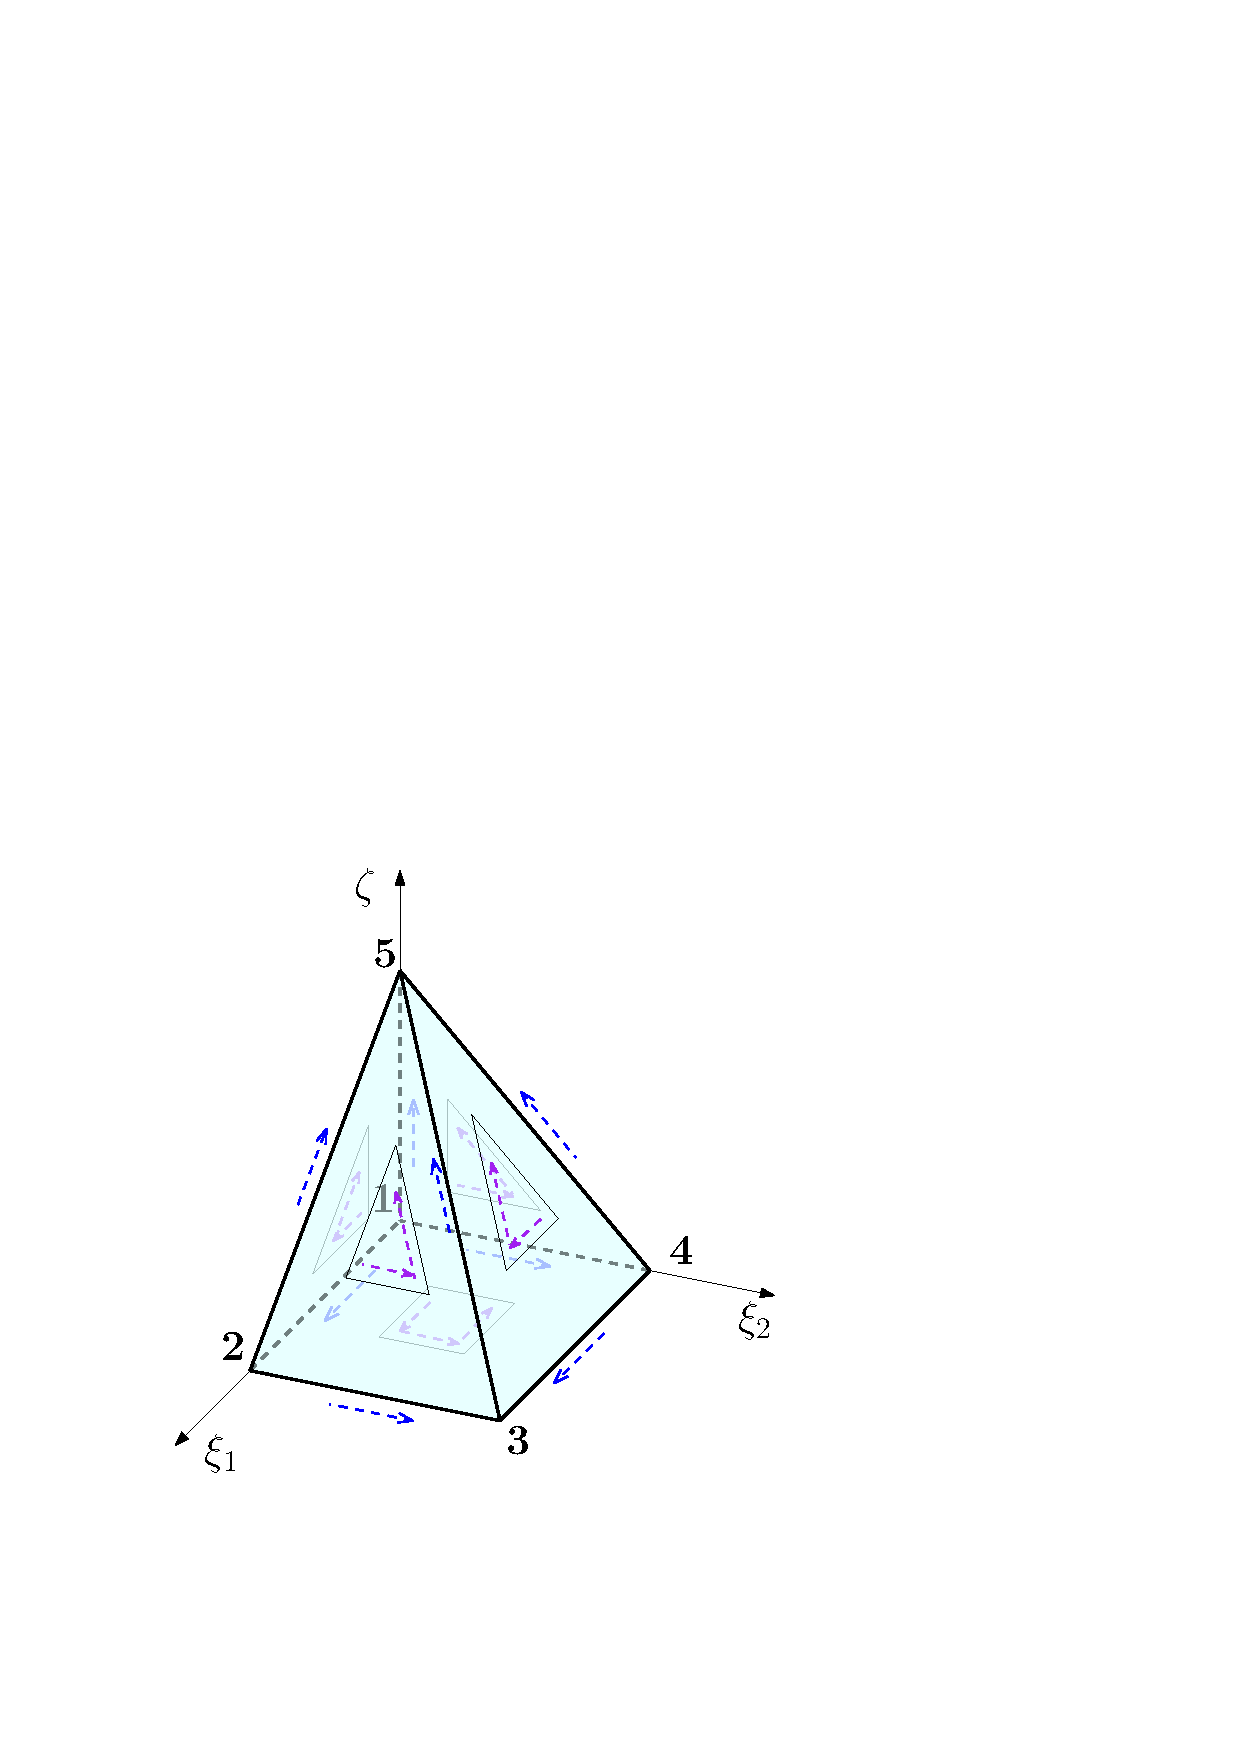
\includegraphics[scale=0.5]{./figures/MasterPyramidOrientations.pdf}
\caption{Master pyramid with numbered vertices \textit{and} local edge and face orientations.}
\label{fig:MasterPyramidOrientations}
\end{center}
\end{figure}

The predefined \textit{local} edge and face orientations for the pyramid are illustrated in Figure \ref{fig:MasterPyramidOrientations}.
They represent the $\oo=0$ case.
The task at hand is to find the associated \textit{locally ordered} tuples of affine coordinates representing those local orientations.
The key is being aware of the relationships between the vertices and the affine coordinates, which have been explained in detail at the beginning of this section. 
Hence, once \S\ref{sec:HexaOrientations}, \S\ref{sec:TetOrientations} and \S\ref{sec:PrismOrientations} are consulted, it should be clear how to construct the orientation embedded shape functions. 
Consult Appendix \ref{app:pyrappendix} if the reader wants to avoid computational instabilities for the $H(\mathrm{div})$ triangle face functions.
